%%%%%%%%%%%%%%%%%%%%%%%%%%%%%%%%%%%%%%%%%%%%%%%%%%%%%%%%%%%%%%%%%%%%%%%%%%%%
% AGUtmpl.tex: this template file is for articles formatted with LaTeX2e,
% Modified July 2014
%
% This template includes commands and instructions
% given in the order necessary to produce a final output that will
% satisfy AGU requirements.
%
% PLEASE DO NOT USE YOUR OWN MACROS
% DO NOT USE \newcommand, \renewcommand, or \def.
%
% FOR FIGURES, DO NOT USE \psfrag or \subfigure.
%
%%%%%%%%%%%%%%%%%%%%%%%%%%%%%%%%%%%%%%%%%%%%%%%%%%%%%%%%%%%%%%%%%%%%%%%%%%%%
%
% All questions should be e-mailed to latex@agu.org.
%
%%%%%%%%%%%%%%%%%%%%%%%%%%%%%%%%%%%%%%%%%%%%%%%%%%%%%%%%%%%%%%%%%%%%%%%%%%%%
%
% Step 1: Set the \documentclass
%
% There are two options for article format: two column (default)
% and draft.
%
% PLEASE USE THE DRAFT OPTION TO SUBMIT YOUR PAPERS.
% The draft option produces double spaced output.
%
% Choose the journal abbreviation for the journal you are
% submitting to:

% jgrga JOURNAL OF GEOPHYSICAL RESEARCH
% gbc   GLOBAL BIOCHEMICAL CYCLES
% grl   GEOPHYSICAL RESEARCH LETTERS
% pal   PALEOCEANOGRAPHY
% ras   RADIO SCIENCE
% rog   REVIEWS OF GEOPHYSICS
% tec   TECTONICS
% wrr   WATER RESOURCES RESEARCH
% gc    GEOCHEMISTRY, GEOPHYSICS, GEOSYSTEMS
% sw    SPACE WEATHER
% ms    JAMES
% ef    EARTH'S FUTURE
% ea    EARTH AND SPACE SCIENCE
%
%
%
% (If you are submitting to a journal other than jgrga,
% substitute the initials of the journal for "jgrga" below.)

\documentclass[draft,ras]{agutex}
\usepackage{graphicx}   
\usepackage{setspace}
\usepackage{amsxtra}
\usepackage{amsmath}
\usepackage{amssymb}
\usepackage{multirow}
\usepackage{bm}
\RequirePackage{lineno}
\linenumbers
% graphics path
\graphicspath{{Figs/}}

% Author names in capital letters:
\authorrunninghead{Swoboda ET AL.}

% Shorter version of title entered in capital letters:
\titlerunninghead{ESA ISR ERRORS}

%Corresponding author mailing address and e-mail address:
%\authoraddr{Corresponding author: A. B. Smith,
%Department of Hydrology and Water Resources, University of
%Arizona, Harshbarger Building 11, Tucson, AZ 85721, USA.
%(a.b.smith@hwr.arizona.edu)}

%% JOHN: REMOVE THIS COMMAND AFTER EDITS ARE DONE
%% mark PJE comments in the text
\newcommand{\pcom}[2]{\marginpar{{\footnotesize \bf #1}}{\it {#2}}}

\begin{document}

%% ------------------------------------------------------------------------ %%
%
%  TITLE
%
%% ------------------------------------------------------------------------ %%


%\title{Trade-Offs Between Statistical Accuracy and Space-Time Resolution in ISR}
\title{Observability of Ionospheric Space-Time Structure with ISR:   A Simulation Study }
%%%%%%%%%%%%%% Author Info %%%%%%%%%%%%%%%%%%%%%%%%%%%%%%%%%%%%%
\authors{John Swoboda,\altaffilmark{1}
Joshua Semeter,\altaffilmark{1} Matthew Zettergren,  \altaffilmark{2} Philip Erickson, \altaffilmark{3}}

\altaffiltext{1}{Department of Electrical \& Computer Engineering,
Boston University, Boston, Massachusetts, USA.}
\altaffiltext{2}{Physical Sciences Department, Embry-Riddle Aeronautical University, Daytona Beach, Florida, USA.}
\altaffiltext{3}{Haystack Observatory, Massachusetts Institute of Technology, Westford, Massachusetts, USA.}
%%%%%%%%%%%%%% Abstract %%%%%%%%%%%%%%%%%%%%%%%%%%%%%%%%%%%%%
%% ------------------------------------------------------------------------ %%
%
%  ABSTRACT
%
%% ------------------------------------------------------------------------ %%

% >> Do NOT include any \begin...\end commands within
% >> the body of the abstract.

\begin{abstract}

The sources of error from electronically steerable array (ESA) incoherent scatter radar (ISR) systems are investigated both theoretically and with use of an open source ISR simulator, developed by the authors, called STISRS (Space-Time ISR Simulator). The main sources of error incorporated in the simulator include statistical uncertainty, which arises due to nature of the measurement mechanism, and the inherent space-time ambiguity from the sensor. The simulator under discussion can take a field of plasma parameters, parameterized by time and space, and create simulated ISR data at the scattered electric field (i.e. complex voltage) level , subsequently processing this data to show possible reconstructions of the parameter field. To demonstrate general utility, we show a number of simulation examples, with one case using data from a self-consistent multi-fluid transport model. Results highlight the significant influence of the forward model of the ISR process and the resulting statistical uncertainty on plasma parameter measurements, and the core trade offs that must be made when planning experiments. These conclusions further point to a need for this type of simulator as a design tool to ease the goal of more optimal experiment design for flexible ESA class ISR systems.


\end{abstract}

%% ------------------------------------------------------------------------ %%
%
%  BEGIN ARTICLE
%
%% ------------------------------------------------------------------------ %%

% The body of the article must start with a \begin{article} command
%
% \end{article} must follow the references section, before the figures
%  and tables.

\begin{article}

\section{Introduction}
Incoherent scatter radar is an important diagnostic for the ionosphere since it yields direct measurements of intrinsic plasma parameters  \citep{dougherty:farley1960, farleydougherty:ISR2, doughteryfarley:ISR3, hagfors1961}. As with all diagnostic tools, though, it has unavoidable measurement uncertainties, including time and spatial ambiguities \citep{farley1969, farleycomppower1969, hysell2008, RDS:RDS20236}.  

One unique aspect of ISR measurements is the use of inherent random fluctuations of the plasma as a remote sensing tool. These fluctuations are processed for information extraction by computing second order statistics, specifically an autocorrelation function (ACF), from a scattered signal \citep{farley1969}. The stochastic nature of the target itself yields the requirement of averaging multiple realizations of the ACF to properly compute a statistical ensemble average, with more averages reducing the variance of the estimate. This forces the assumption of wide-sense stationarity for a space-time cell, which may not always be true. In the context of experiment design, this creates a trade-off between space-time resolution and the variance of the measurements.

Application of electronically steerable array (ESA) technology to ISR has been a recent community advancement. ESA capable ISRs, such as the Advanced Modular Incoherent Scatter (AMISR) systems, have already been deployed in Poker Flat Alaska and Resolute Bay Canada \citep{Nicolls:2007ie, dahlgren2012di}. ESA based systems are seen as the future of the ISR sensor modality due to the flexibility in beam steering and processing over single antenna based systems. The next step in the evolution of these systems is the EISCAT-3D project, which is expected to have a number of enhancements such as multi-static processing capability.

One benefit of ESA based ISR is that volumetric reconstructions of plasma parameters can be created \citep{Semeter2009738, Nicolls:2007ie, dahlgren2012di}. ESA systems also have been used to reconstruct full vector velocity fields from line-of-sight bulk Doppler measurements \citep{butler:imagingfregiondrifts,RDS:RDS20195}. However, it has been shown that volumetric reconstructions of this type can yield measurements with a high degree of parameter ambiguity \citep{Dahlgren:2012dq}. Similar types of ambiguities arise using systems with a single antenna.  \citet{Semeter:2005fo} illustrated the challenges in interpreting spatially scanned measurements in a highly dynamic environment, as well as the benefits of a flexible post-processing environment.

With the continued interest in ISR as an imaging sensor, 
a rigorous mathematical framework is needed to understand uncertainties in the high-level data products produced.  These sources of error, from statistical uncertainty and spatio-temporal ambiguity, create complex functions and choices in the context of experiment design. Because of this complex multi-dimensional trade space, it is useful to simulate the ISR measurement process before an experiment is attempted. 
% JOHN:  Experiment design is only a part of the story.   What I write below is really talking about a Bayesian assimilation framework.  Do you agree?  We can discuss whether to expand further for this paper.
ISR is also increasingly called upon to validate predictions from multi-dimensional physical models.  Simulation becomes a critical tool in this  context by providing a quantitative assessment of the observability of a predicted response, which involve subtle variations in ionospheric state parameters (see Section~\ref{sec:fullparam}).  

This paper describes a method to simulate the entire ISR process with consideration of all three spatial sampling dimensions for a monostatic radar. This method is available in the software package called STISRS (Space-Time ISR Simulator).  The remainder of paper is organized as follows. Section 2 will list possible sources of ISR error, which are included in our simulation method. The simulation method behind STISRS will be described in Section 3. Section 4 will show a number of examples of from the simulator, ranging from a stationary column of enhanced electron density to the output of a self-consistent multi-fluid ionospheric model \citep{semeter:plasmatransport2012}. These examples point the way towards development of best practices for systematic ESA class ISR experiment design intended to conduct measurements that best reflect the physics actually present in the ionosphere.
%%%%%%%%%%%%%%%%%%%%%%%%%%%%%%%%%%%%%%%%%%%%%%%%%%%%%%%%%%%%%%%%%%%%%%%%%%%%%%%%%%%%%%%%%%%%%%
\section{ISR Errors}

In this section two sources of ISR error will be discussed. The first part of this discussion will cover the statistical uncertainty that arises from the ISR measurement process. Following this, the errors originating from both the spatial and temporal ambiguity of ISR experimental systems will be shown. The goal is to develop a more fully realized foundation for the trade-offs that must be considered by the ISR experiment designer for a given science application.

\subsection{Statistical Errors}

The electron density fluctuations observed by ISR techniques are associated primarily with two longitudinal wave modes in the plasma: the ion-acoustic mode and the Langmuir mode \citep{evans;isr}.  Most ISR experiments involve the use of multiple independent samples, created by measuring ionospheric scatter from repeated individual radar pulses, to create an estimate of the ion acoustic spectrum (i.e., the Fourier transform of the autocorrelation function or ACF). This experimental observation is then fit to a theoretical plasma physics based model in order to estimate ionospheric state parameters (typically plasma density, electron temperature, ion temperature, and bulk line-of-sight plasma motion). The theory or how the plasma parameters impact the statistics of the density fluctuations has developed through in a series of studies since the first use of this sensor modality \citep{gordon58,dougherty:farley1960, farleydougherty:ISR2, doughteryfarley:ISR3, hagfors1961}, with reformulations of the theory occurring even recently  \citep{kudeki:milla:1,kudeki:milla:2}. 

The two main sources of statistical uncertainty in received electric field fluctuations within radar backscatter, or, equivalently, in received voltages measured at the antenna terminals of a radar system, are described here as (1) random fluctuations from the electron density, and (2) noise from within the sensor itself. There are other sources of increased uncertainty, including sky noise and coherent scatter from other targets, but that is outside the scope of this paper.
% JOHN:  don't sky noise and receiver noise propagate identically thru the math?   Just wondering about the "outside the scope" comment.  The coherent scatter from other targets is clutter, which is a different category.

The received voltage values at the antenna terminal, comprising the incoherent scatter signal, also have the properties of a random process. As such, it is necessary to average samples of an estimator for autocorrelation or power spectrum \citep{Diaz:2008co}.  For the autocorrelation case, a covariance matrix between each lag estimate can be determined using the formulation in Equation 2 of \citet{hysell2008}, rewritten here as

\begin{equation}
\label{eqn:covcalc}
C_{\tau_1,\tau_2} = \frac{1}{2J} \left( \ R(0)  R^*(\tau_1-\tau_2) +  R(\tau_1) R^*(\tau_2) \right),
\end{equation}

\noindent where, $R(\tau)$ is the estimated ACF as a function of lag $\tau$, $C_{\tau_1,\tau_2}$ is the entry in the covariance matrix of the estimated ACF at lags $\tau_1$ and $\tau_2$,  and $J$ is the number of samples or pulses averaged together to create the estimate. The diagonals of this matrix can be thought of as the autocovariances of each of the lags.  Thus, by setting $\tau_2 = \tau_1 \equiv \tau$, Equation \ref{eqn:covcalc} simplifies to

\begin{equation}
\label{eqn:covdiag}
C_{\tau,\tau} = \frac{1}{2J} \left(  |R(0)|^2 +|R(\tau)|^2\right).
\end{equation}

The variance of this signal is further increased once noise from the sensor is added.  If the noise from the sensor is assumed to be uncorrelated to the signal, the error from the noise, $\left|R_w (\tau)\right|^2$, the square of the noise ACF, can simply be added to the error from the inherent fluctuations in the signal,


\begin{equation}
\label{eqn:covdiagwn}
C_{\tau,\tau} = \frac{1}{2J} \left(  |R(0)|^2 +|R(\tau)|^2 + \left|R_w (0)\right|^2+\left|R_w (\tau)\right|^2\right).
\end{equation}

\subsection{Space-Time Errors}

For practical radar experiments, the use of waveforms with non-zero time extent introduces artifacts in the form of an associated radar ambiguity function \citep{nygren1996}.  The errors created through this ambiguity function lead to a blurring or averaging of ACFs from different points in time and space. This is analogous to a blurring operator one might encounter in standard image processing applications.
 
The space-time ambiguity, $L(\tau_s,\mathbf{r}_s,t_s,\tau,\mathbf{r},t)$, is the kernel of a Fredholm integral equation of the first kind operating on the ACF, $R(\tau,\mathbf{r},t)$, which can change over space, $\mathbf{r}$, and time $t$. It can be represented as follows,

 \begin{equation}
  \label{eqn:staf}
  \rho(\tau_s,\mathbf{r}_s,t_s) =\int L(\tau_s,\mathbf{r}_s,t_s,\tau,\mathbf{r},t)R(\tau,\mathbf{r},t)dVdtd\tau,
\end{equation}

\noindent where the subscript $s$ delineates the variable as the discretized version of its continuous counter part--i. e., the variable $\tau_s$ is the sampled version of $\tau$ representing lag. 

\citet{RDS:RDS20236} showed that the general ambiguity kernel is a separable function when the spatial coordinates are spherical, where ($r,\theta,\phi)$ represent, range, azimuth and elevation respectively.  In this case, Equation \ref{eqn:staf} becomes

\begin{equation}
\label{eqn:stafbrok}
\rho(\tau_s,\mathbf{r}_s,t_s)= \int G(t_s,t)F(\theta_s,\phi_s,\theta,\phi)W(\tau_s,r_s,\tau,r) R(\tau,\mathbf{r},t) dVdt d\tau,
\end{equation}

\noindent where $G(t_s,t)$ is the kernel for the time dimension, $F(\theta_s,\phi_s,\theta,\phi)$ is radar beam shape which acts as a kernel in azimuth and elevation, and $W(\tau_s,r_s,\tau,r) $ represents the range-lag ambiguity function which acts as a kernel along range $r$ and lag $\tau$. The derivation of this operator is also given by \citet{RDS:RDS20236}.

For ISR experiment design, both the radar beam ambiguity and range-lag ambiguity functions create a fundamental trade off between statistical variation of the signal and spatiotemporal resolution of the signal. In order to perform a statistical estimate of signal fluctuations, radar pulses (each a separate sample of the overall statistical process) need to be averaged together. Due to the statistical nature of ISR radar scatter, this is necessary even for the case of infinite signal-to-noise ratio.   

The statistical averaging process is mainly done over time, but can be done over space as well by averaging across beams or range gates. If the ionosphere is drifting with a known vector velocity, \citet{RDS:RDS20236} pointed out that the stationarity assumption for ISR integration is  better met by averaging those beam positions that approximately correspond to the same scattering volume within the moving frame of reference. However, this approach may degrade spatial resolution at the expense of improvement in temporal resolution. 
%As tradeoffs similar to these are inherently coupled and often case-specific, the best approach for a given experimental situation can best be explored through simulation.
The optimal experiment design and processing strategy depend critically on the objectives of the experiment.   This trade space may be effectively explored through simulation.

%%%%%%%%%%%%%%%%%%%%%%%%%%%%%%%%%%%%%%%%%%%%%%%%%%%%%%%%%%%%%%%%%%%%%%%%%%%%%%%%%%%%%%%%%%%%%
\section{Simulation Methodology}

The following section will detail the processing steps in STISRS. It allows one to analyze different general ISR experiment scenarios by simulating the ISR measurement process. The space-time ambiguity is modeled using a coordinate transform and the pulse as a window along range while the statistical error is taken into account by creating complex shaped Gaussian noise.  We begin with a description of construction of spectral filters designed to create the noise-like signal received in ISR experiments. This is followed by description of the process of creating complex receiver voltage data. The last portion will detail the processing used to create statistical estimates of ACFs.

\subsection{Creating Filters}

The simulator takes as input a discretized set of ionosphere state parameters in Cartesian coordinates which can vary in time.  This corresponds to the true field we seek to reconstruct. The first step in the simulator is to create theoretical ISR spectra at each point from the prescribed parameters. For details on calculating these spectra from the intrinsic plasma parameters see, e.g., \citet{kudeki:milla:1} and \citet{kudeki:milla:2}. 

Once the spectra have been created, the simulator transforms the resulting values to a radar-centered spherical coordinate system. This coordinate change acts as a linear operator in spatial dimensions, and the spectra are accordingly weighted and averaged. The weighting in azimuth and elevation is determined by the antenna beam pattern, while the weighting in range (i.e. along beam) is simply a binary test of whether the spectra are within the range gate. If there are no spectra within the range gate, a nearest neighbor rule is used which selects the closest point in Cartesian space. This method to create the spectra for each point is an acceptable approximation because spatial correlations between the electron density fluctuations will be on the order of the Debye length \citep{farley1969}, which is in nearly all practical cases significantly smaller than the beam width or range gate size. The algorithm implementing spatial sampling is shown in the simplified diagram in Figure \ref{fig:beamdia}.

\begin{figure}[!t]
\centering
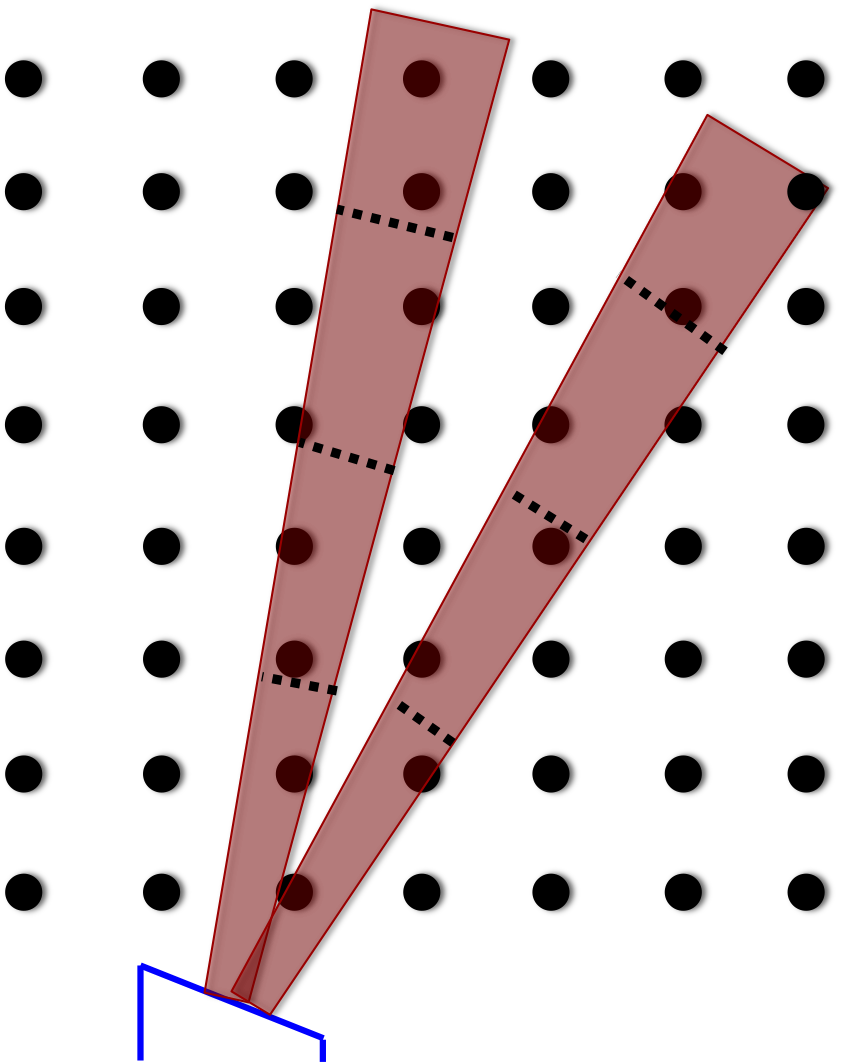
\includegraphics[width=2in]{beamsampling}
\caption{Each point is a from a discrete sampling of a Cartesian space. The beams are broken up into range gates, separated by the dotted lines, and the parameters at each point overlapping within these gates are averaged.}
\label{fig:beamdia}
\end{figure}
 
% Once the spectrum at the specific point in range and angle space has been determined, the filter $H_m(\omega)$, is created by simply taking the square root of the spectrum, $S_m(\omega | \: \bm{\theta})$,

% \begin{equation}
% \label{eq1}
% H_m(\omega) = \sqrt{S_m(\omega | \: \bm{\theta})}.
% \end{equation}

Once the theoretical spectrum for a given scattering volume has been calculated, an appropriate spectral shaping filter is created. The method to create the filter given a desired spectrum or ACF can be done in a number of ways \citep{Kasdin:1995wi}. The implementation in STISRS creates an infinite impulse response filter. The coefficients are determined using the ACF by solving the following set of equations,

\begin{equation}
\label{eq:filtereq}
\begin{bmatrix} R_m(0) & R_m(1)& \cdots & R_m(L-1) \\ R_m(L-1) & R_m(0)& \cdots & R_m(L-2)\\ \vdots & &\ddots  & \vdots \\  R_m(1) & R_m(2) & \cdots & R_m(0) \end{bmatrix} \left[ \begin{array}{c} a_1\\ a_2\\\vdots \\ a_L \end{array} \right]=\left[ \begin{array}{c} R_m(1) \\ R_m(2)\\ \vdots \\R_m(L) \end{array} \right]
\end{equation}

\noindent where $R_m(l)$ are the ACF values, $L$ is the desired length of the filter, and $ a_i$ are the set of filter coefficients. The filter then takes the form in the frequency domain as the following,

\begin{equation}
\label{eq:filtz}
H_m(z) = \frac{G}{1-\displaystyle \sum_{l=1}^{L} a_l z^{-l}}.
\end{equation}
\noindent The gain term $G$ is used to make sure the noise has the correct variance. This can be calculated as 

\begin{equation}
\label{eq:gainterm}
G=\sqrt{\displaystyle \sum_{l=0}^L -a_l R_m(l)},
\end{equation}

\noindent where $a_0=-1$.  This method has been used in similar ways in other contexts, e.g. the creation of vocoders for speech processing applications \citep{rabinerdigitalspeech}.
%\noindent The term $ \bm{\theta}$ refers to the plasma parameters needed to make the spectrum. This filter then is used to create the synthetic IQ data.

\subsection{Simulated Complex Voltage Creation}

The algorithm used to create sampled complex receiver voltages employs a complex white Gaussian noise (CWGN) process (``plant") that is spectrally shaped at its output using a time domain filter. As stated in the previous subsection, each point in space and time will have a separate noise plant and filter which is derived from the plasma and radar parameters parameters.  Figure \ref{fig:IQdiagram} presents a representative example. 

\begin{figure}[h!]
\centering
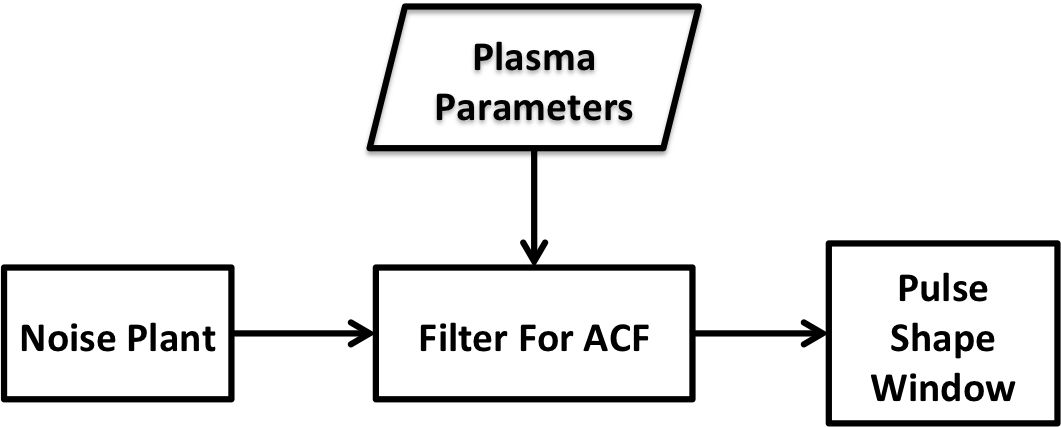
\includegraphics[width=4in]{diagrampart}
\caption{Diagram for complex receiver voltage simulator signal flow.}
\label{fig:IQdiagram}
\end{figure}

The creation of one set of complex receiver voltage data can be represented by

\begin{equation}
\label{eq2}
y_m (k)= s(k)\left[h_m(k)*w(k)\right],
\end{equation}
 
\noindent where $s(k)$ is the overall transmitted pulse envelope, $h_m(k)$ is the time domain representation of the filter in Equation \ref{eq:filtz} and $w(k)\sim CN(0,\mathbf{I})$ or CWGN noise process. The pulse shape acts as a window, since the plasma will only reflect energy during the time it is illuminated by the radar signal. 
%The application of this filter is actually done in the frequency domain. This is possible because the Discrete Fourier Transform (DFT) of a vector of CWGN is also CWGN. The only difference is that there is a change in the variance, which is tied to the number of points used in the DFT \citep{kayvol1}. With this in mind Equation \ref{eq2} can be implemented as the following,

%\begin{equation}
%\label{eq:fftfilt}
%y_m (k)= s(k)\displaystyle \sum_{i=0}^{K-1}e^{j\omega_ik}\left[ \sqrt{S_m(\omega_i | \: \bm{\theta})}w(\omega_i)\right],
%\end{equation}
%
%\noindent where $\omega_i$ is the frequency variable, $w(\omega_i) \sim CN(0,\mathbf{I})$ and $K$ is the number of points used for the DFT \citep{michellnoisesim1981}.

\begin{figure}[!h]
\centering
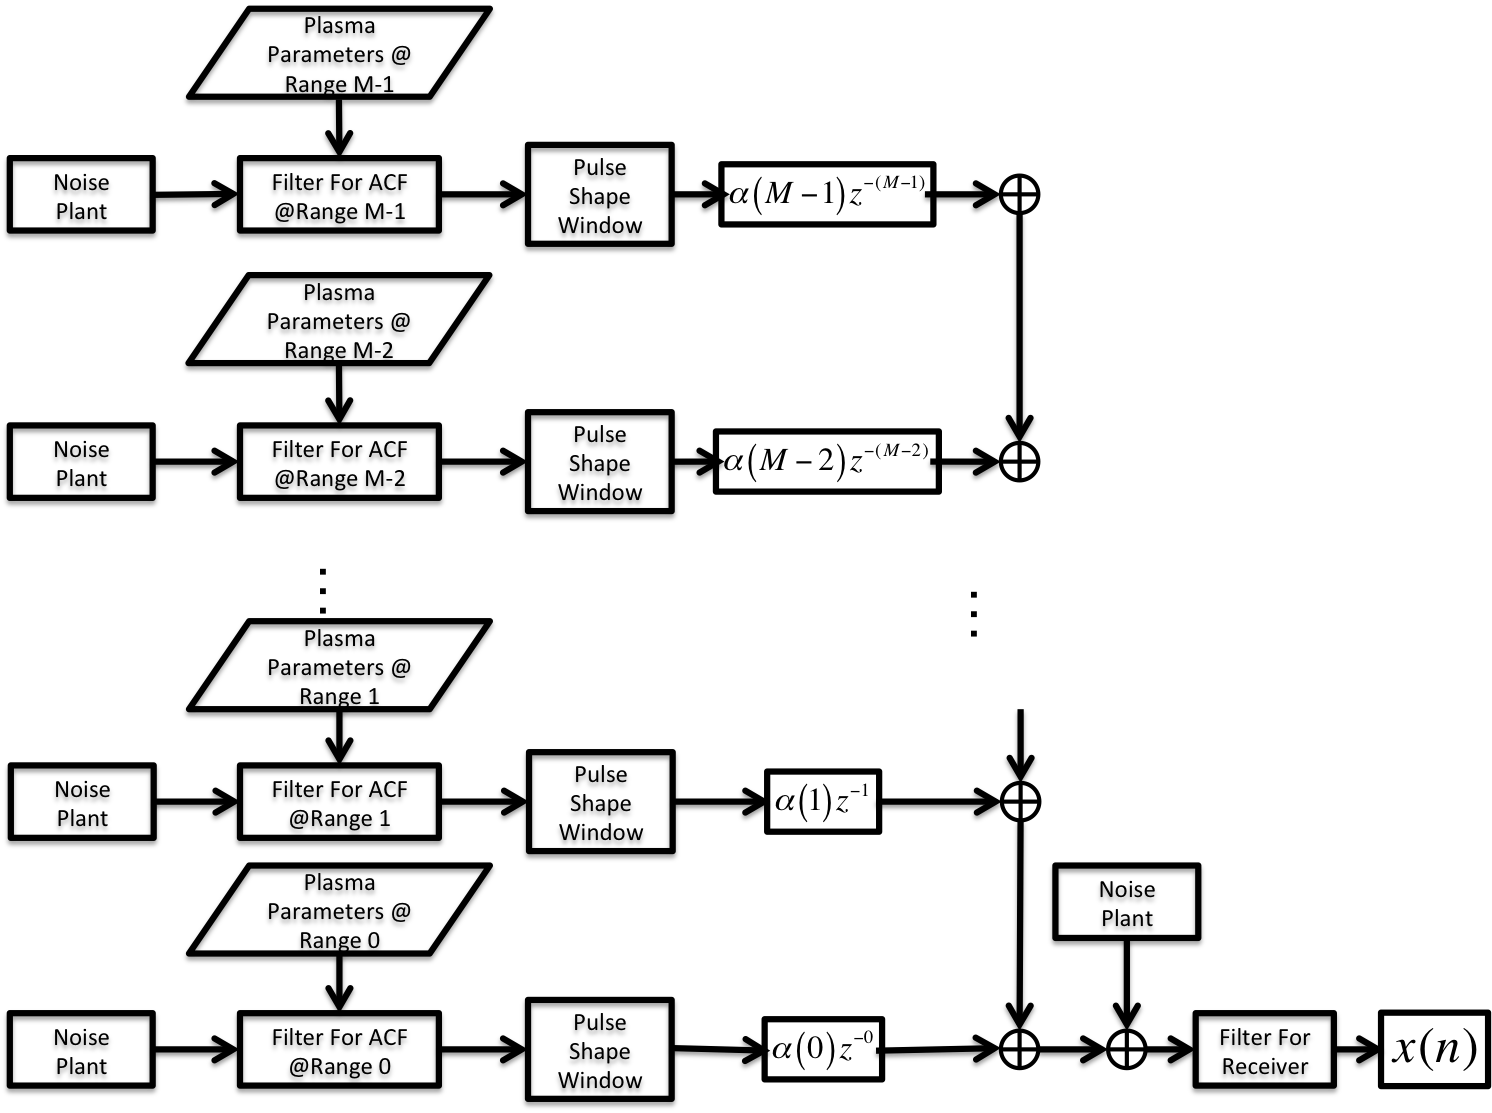
\includegraphics[width=7.0in]{diagram}
\caption{ISR simulation diagram.}
\label{fig:isrdiag}
\end{figure}


After the data for each range gate $y_m(k)$ is created, the received signal's power spectrum can be calculated from ISR plasma scattering theory as 

\begin{equation}
\label{eq3}
P_r = \frac{cG \lambda^2}{2(4\pi)^2}\frac{P_t }{R^2}\frac{\sigma_e N_e}{(1+k^2\lambda_D^2),(1+k^2\lambda_D^2 + T_r)},
\end{equation}
 
 \noindent where $P_r$ is the power received in Watts (W), $k$ is the wavenumber of the radar in meters (m), $c$ is the speed of light in m/s, $G$ is the gain of the antenna, $P_t$ is the power of the transmitter in W, $\sigma_e$ is the electron radar cross section in $m^2$,  $\lambda_D$ is the Debye length in m, $N_e$ is the electron density in m$^{-3}$and $T_r$ is the electron to ion temperature ratio.
  
The received signal power calculated at each range gate using Equation~\ref{eq3} is used as a scaling constant for each $y_m(k)$ series.  Finally, a delayed and summed operator yields a model of the received radar scatter signal:
 
\begin{equation}
\label{eq4}
x(n) = \displaystyle\sum\limits_{m =0}^{M-1} \alpha(m)y_m(n-m),
\end{equation}

\noindent where $\alpha(m) = \sqrt{P_r(m)}/\widehat{\sigma}_y$ and $\widehat{\sigma}_y$ is the estimate of the standard deviation of $y_m(k)$. Lastly, to model total noise from the radar system and environment, an additive CWGN process is included, creating the final simulated complex receiver voltage sequence

\begin{equation}
\label{eq:addnoise}
x_f(n) = x(n) +\sqrt{\frac{k_bT_{sys}B}{2}} w(n), \quad w(k)\sim CN(0,\mathbf{I})
\end{equation}

\noindent where $k_b$ is Boltzmann's constant, $T_{sys}$ is the system temperature and $B$ is the system bandwidth.
A full diagram of the model can be seen in Figure \ref{fig:isrdiag}.


\subsection{ACF Estimation}

After complex receiver voltage data has been created, it is processed to create estimates of the ACF at desired points of space \citep[see, e.g.,][]{farley1969,nygren1996}. This processing follows the flow chart presented in Figure \ref{fig:chain}.  Note that we assume here a signal pipeline which creates a single altitude measurement for analysis.  More sophisticated approaches for ISR analysis exist that use information from multiple altitudes, including full profile analysis \citep{RDS:RDS3308}, lag profile inversion \citep{Virtanen:20082vx}, and others, but treatment of these approaches is beyond the scope of this work.

\begin{figure}[!t]
\centering
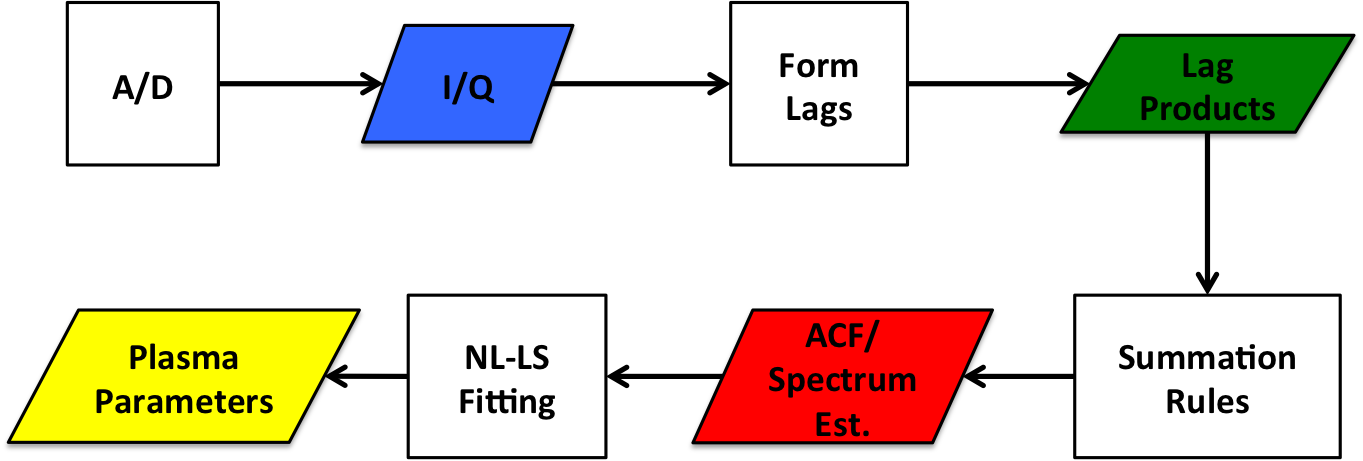
\includegraphics[width=6in]{datastackchain}
\caption{ISR signal processing chain, with signal processing operations as squares and data products as diamonds.}
\label{fig:chain}
\end{figure}


The lag product formation is an initial estimate of the autocorrelation function. The sampled complex receiver voltage can be represented as $x(n) \in\mathbb{C}^N$ where $N$ is the number of samples in an inter pulse period. For each range gate $m\in 0,1,...M-1$ a complex autocorrelation is estimated for each lag of $l \in 0,1...,L-1$.  To get better statistics this operation is performed for each pulse $j\in 0,1,...J-1$ and then summed over $J$ independent pulses. The entire operation to form the initial estimate of $\widehat{R}(m,l)$ may be expressed as

\begin{equation}
\label{eq:lagpro}
\widehat{R}(m,l) = \displaystyle\sum\limits_{j=0}^{J-1} x(m-\lfloor l/2\rfloor,j)x^*(m+\lceil l/2 \rceil,j).
\end{equation}

The case shown in Equation \ref{eq:lagpro} is a centered lag product.  Other types of lag product calculations are available but generally a centered product is used. In the centered lag product case range gate index $m$ and sample index $n$ can be related by $m=n-\lfloor L/2\rfloor$ and the maximum lag and sample relation is $M=N-\lceil L/2 \rceil$.  This lag product formation is the first step in taking a discrete Wigner Distribution \citep{TFAcohen}. This first step adds a bias to the ACF estimate which acts as a weighting on larger lags, represented as $\mathcal{W}(l)$ where weighting can be calculated from details of the range-lag ambiguity function along the range axis. The expected value for the estimator, assuming the use of a simple uncoded pulse waveform, becomes

\begin{equation}
\label{eq:lagprobias}
\left\langle\widehat{R}(m,l) \right\rangle = \mathcal{W}(l)R(m,l) =\frac{L-l}{L}R(m,l).
\end{equation}
%This specific type of lag product formation is detailed in \citep{farley1969} and had been referred to as unbiased. This terminology does differ from what is used in statistic signal processing literature such as \citep{randomsigshanmugan} where the unbiased autocorrelation function estimate is carried out as so,
%
%\begin{equation}
%\label{eq:lagproub}
%\hat{R}(m,l) = \frac{1}{L-l}\displaystyle\sum\limits_{j=0}^{J-1} x(m-\lfloor l/2\rfloor,j)x^*(m+\lceil l/2 \rceil,j).
%\end{equation}
%
%\noindent With out the $\frac{1}{L-l}$ term the estimator will be windowed with a triangular function thus impacting the estimate of the ISR spectrum as this will act as a convolution in the frequency domain. This bias is taken into account in \citep{farley1969} but it is simply wrapped up into the ambiguity function. 

Applying a summation rule is generally the next step in creating an estimate of the autocorrelation function for single altitude analysis. This is done for a number of reasons, but primarily to improve estimate statistics.  Furthermore, if the right rule is chosen, then the range ambiguity can be made approximately constant across the lags \citep{nygren1996}. 
% JOHN:  the use of a summation rule is intimately connected to the "overspread" issue, which leads to redundant entries in the lag profile matrix, right?   I've not thought about it deeply, but I wonder if we can say something insightful about this here.  As far as I know, summation rule issues haven't been discussed in the literature in detail.
The trapezoidal summation rule used in our simulation is a common choice and can be represented as follows.

\begin{equation}
\label{eq:sumrule}
\widehat{R}_s(m,l) = \displaystyle\sum\limits_{i=-((v-1)/2+\lceil l/2 \rceil)}^{((v-1)/2+\lfloor l/2\rfloor)} \widehat{R}(m+i,l),
\end{equation}

\noindent where $v$ is the 'volume' index or the number of gates integrated at zero lag (restricted to odd integers here) and $\widehat{R}_s(m,l)$ is the final ACF estimate after the summation rule \citep{nygren1996}. 
% pcom checked for variables, already defined
However, the final result of this summation rule will still lead to a biased ACF. For the uncoded waveform case, this summation rule leads to the ollowing expected value for the estimator \citep{nygren1996},

\begin{equation}
\label{eq:sumruleest}
\left\langle\widehat{R}_s(m,l) \right\rangle  =\frac{v+l}{v\mathcal{W}(0)}\mathcal{W}(l)R(m,l) =\left(-\frac{1}{vL}l^2+\frac{L-v}{Lv}l+1\right)   R(m,l).
\end{equation}
%An example summation rule for a central product is shown in Figure \ref{fig:sumrule}. In the figure the image on the left is a basic representation of an ambiguity function of a long pulse.  Its mirrored on the right with red bars which would show the integration area under it so the ambiguity function for each lag will be of equal size in range. There are a number of different summing rule each with their own trade offs \citep{nygren1996}.

%In the processing this is basically a summing of lags from different ranges. The amount of summing is similar to what is shown in Figure \ref{fig:sumrule}.   



%\begin{equation}
%\label{eq:lagpronoise}
%\hat{R}_w(m,l) = \displaystyle\sum\limits_{j=0}^{J-1} w(m_w-\lfloor l/2\rfloor,j)w^*(m_w+\lceil l/2 \rceil,j),
%\end{equation}

Finally, noise effects are included by subtracting an estimate of the noise correlation from $\widehat{R}_s(m,l)$.  We represent the noise correlation function as $\widehat{R}_w(m,l)$, the ACF estimate of the background noise process of the radar $w(n_w)$ using the steps in Equations \ref{eq:lagpro} and \ref{eq:sumrule}. In a real radar system the noise process is typically sampled either during a calibration period for the radar when nothing is being emitted, or at ranges sufficiently distant that scattered ionospheric signal is assumed to be negligible. For our simulated estimate, we simply use a noise process with the same correlation structure and power as the noise that was added. The final estimate of the autocorrelation function after the noise subtraction and summation rule is represented by $\widehat{R}_f(m,l)$.

%\begin{figure}[!t]
%\centering
%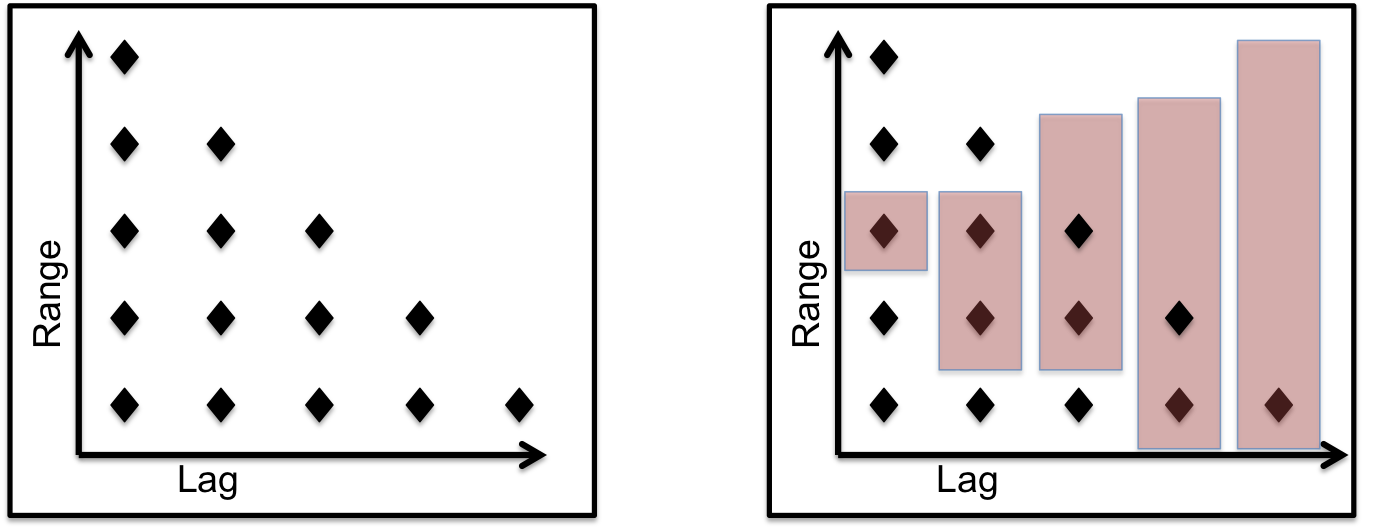
\includegraphics[width=3in]{sumrule}
%% where an .eps filename suffix will be assumed under latex, 
%% and a .pdf suffix will be assumed for pdflatex; or what has been declared
%% via \DeclareGraphicsExtensions.
%\caption{Summation Rule Diagram}
%\label{fig:sumrule}
%\end{figure}

After the final estimation of the spectrum is complete, nonlinear least squares fitting takes place to determine plasma parameters.  
%\pcom{This entire section can be collapsed to one reference and saved for the thesis chapter.}%
%{
The class of nonlinear least squares problems relevant to ISR parameter estimation can be represented as the minimization of a cost function of the form \citep{kayvol1},

\begin{equation}
	\mathbf{\hat{p}}= \underset{\mathbf{p}}{\text{argmin}} (\mathbf{y}-\bm{\theta}(\mathbf{p}))^*\bm{\Sigma}^{-1}(\mathbf{y}-\bm{\theta}(\mathbf{p})).
\label{nlls}
\end{equation}

In Equation \ref{nlls}, the data represented as $\mathbf{y}$ would be the final estimate of the ACF $\widehat{R}_f(m,l)$ at a specific range, or its spectrum $\widehat{S}_f(m,\omega)$. The parameter vector $\mathbf{P}$ would be the plasma parameters $N_e$, $T_e$, $T_i$ and $V_i$. The fit function, $\bm{\theta}$, is the IS spectrum calculated from a models \citep[e.g.,][]{kudeki:milla:1} and smeared by the ambiguity function. In the case of the long pulse the ambiguity can be simply applied by multiplying it with the autocorrelation function $R(l)$ if the summation rule is properly applied. In the past, the Levenberg-Marquart algorithm to fit data \citep{nikoukar2008}.
% JOHN:  I may have missed something, but what are you using to fit the data (i.e., for the nonlinear minimization)?


%Using the covariance matrix from the fitted parameters, an overall error estimate can be achieved. This matrix is calculated using a numerical approximation to the Jacobian matrix that the function uses to determine the solution. Due to the way the numerical routines solve the problem, this matrix must be multiplied by the error between the estimated parameters and the data,

The last step is to calculate the errors in the parameter estimates. In order to do this a numerical approximation of the jacobian matrix between the data and the ACF, $\mathbf{J}$, at $\mathbf{p}=\mathbf{\hat{p}}$. The formula to estimate the parameter error matrix, $\mathbf{C}_{\mathbf{\hat{p}}}$ according to \citet{Hysell:2000cq}, is


\begin{equation}
\label{eqn:jacinv}
\mathbf{C}_{\mathbf{\hat{p}}}=(\mathbf{J}^T \mathbf{C}^{-1}\mathbf{J})^{-1},
\end{equation}
%\begin{equation}
%\label{eqn:jacinv}
%\bm{\Sigma}_{\mathbf{\hat{p}}}=\frac{(\mathbf{J}^T\mathbf{J})^{-1} (\mathbf{y}-\bm{\theta}(\mathbf{\hat{p}}))^*\bm{\Sigma}^{-1}(\mathbf{y}-\bm{\theta}(\mathbf{\hat{p}}))}{L-N_{\mathbf{p}}},
%\end{equation}

\noindent where $ \mathbf{C}$ is the covariance matrix from the ACFs or spectra depending on what is being fit. The covariance matrix for the ACF is detailed in Equation \ref{eqn:covcalc}, while the covariance matrix of the spectra is simply the ACF matrix but with discrete Fourier Transforms applied to the rows and columns. The variances of the parameters are then taken as the diagonals of the matrix.


%The correlation matrix $\bm{\Sigma}$ is often realized as a diagonal matrix for many ISR systems the variance of the lags or each point of the spectrum being the values. The variance of the ACF estimator can be estimated using the following,
%
%\begin{equation}
%\label{eqn:acfvar}
%\sigma_{\hat{R}(l)}^2=\frac{1}{JL}\displaystyle \sum_{m=-(L-l-1)}^{L-l-1}\left(\frac{L-|m|+1}{L}\right)\left(|\hat{R}(m)|^2 +|\hat{R}(m+l)\hat{R}(m-l)|\right) + \hat{N}^2
%\end{equation}
%
%\noindent where $N$ is the estimated noise power. To estimate the spectrum variance the matrix $\bm{\Sigma}$ is transformed in to the Fourier domain using FFTs (FFT on the columns and IFFT on the rows) so as to model the $\mathbf{F}\bm{\Sigma} \mathbf{F}^*$ matrix operation. 



%%
%The diagonal values usually used, noted as $\sigma_i^2$, usually the same unless there is a larger measurement error for one of the lags or spectrums.  The following formula from  \citep{nicollsisrschool2013} can be used:

%\begin{equation}
%\label{sigpow}
%\sigma_i = \frac{S}{\sqrt{J}}\left(1+\frac{1}{SNR}\right).
%\end{equation}

%\noindent where $S$ is the signal power and $SNR$ is the signal to noise ratio. The noise level can be estimated from the calibration period. 

%In the past, ISR researchers have used the Levenberg-Marquart algorithm to fit data \citep{nikoukar2008}. This specific iterative algorithm moves the parameter vector $\mathbf{p}$ by a perturbation $\mathbf{h}$ at each iteration\citep{gavin:2013}. Specifically Levenberg-Marquart was designed to be a sort of meld between two different methods Gradient Decent, and Gauss-Newton. The perturbation vector $\mathbf{h}_{lm}$ can be calculated using the following:
%
%\begin{equation}
%\left[ \mathbf{J}^T\bm{\Sigma}^{-1}\mathbf{J}\right]\mathbf{h}_{lm} =\mathbf{J}^T\bm{\Sigma}^{-1}(\mathbf{y}-\bm{\theta}(\mathbf{p}))
%\label{hlm}
%\end{equation}
%
%\noindent where $\mathbf{J}$ is the Jacobian matrix $\partial \bm{\theta}/\partial \mathbf{p}$ \citep{levenberg1944,marquardt:1963}. 
%
%Using the covariance matrix from the fitted parameters, an overall error estimate can be achieved. This matrix is calculated using a numerical approximation to the Jacobian matrix that the function uses to determine the solution. The Hessian, $\mathbf{H}$ is then calculated by using the Jacobian and then inverted to get the covariance matrix. Due to the way the numerical routines solve the problem, this matrix must be multiplied by the error between the estimated parameters and the data,
%
%\begin{equation}
%\label{eqn:jacinv}
%\bm{\Sigma}_{\mathbf{\hat{p}}}=\frac{(\mathbf{J}^T\mathbf{J})^{-1} (\mathbf{y}-\bm{\theta}(\mathbf{\hat{p}}))^*\bm{\Sigma}^{-1}(\mathbf{y}-\bm{\theta}(\mathbf{\hat{p}}))}{L-N_{\mathbf{p}}},
%\end{equation}

%\noindent where $N_{\mathbf{p}}$ is the number of parameters being fit. The variances of the parameters are then taken as the diagonals of the matrix.}

 %If the Hessian matrix is undefined so it can not be inverted and a proper estimate of the errors is not possible.

%%%%%%%%%%%%%%%%%%%%%%%%%%%%%%%%%%%%%%%%%%%%%%%%%%%%%%%%%%%%%%%%%%%%%%%%%%%%%%%%%%%%%%%%%%
\section{Simulation Examples}
The framework for STISRS allows exploration of a number of aspects of ISR processing. Within the scope of this article, we will focus on three application examples.

The first example demonstrates how the simulator can be used for Monte Carlo estimates of ISR spectra. In this case, we hold all of the plasma parameters constant and determine how the distribution of the measured parameters evolve. The next example uses a simple altitude distribution of ionospheric plasma parameters to show the impact of the forward model of the ISR on a basic measurement of electron density. This is intended to illustrate that basic ambiguities inherent in ISR measurements can give the appearance of a change in morphology of the plasma phenomena when none truly exists. Finally, the output of a fully consistent multi-fluid ionosphere model is used as input to the ISR simulator to show a use case relevant to experiment planning. This case illustrates an inherent tradeoff in experiment construction between reducing statistical fluctuations in the measurement and increasing distortion in the final reconstruction.

\subsection{Monte Carlo Example}

It is often necessary to get a large number of sensor measurements for a statistical study or perhaps create a training data set for a pattern recognition algorithm. This can require large amount of work by the researcher to search and classify the different data. Fortunately there may be cases where one could use STISRS to create some synthetic data instead.

%\pcom{Very awkward and verbose; rewrite}{It is necessary to understand the statistics from the sensors used in scientific studies. In order to do this a large number of measurements must be taken with the sensor. There are issues with this approach in that the inputs can not be controlled so along with any random variation that may be found in the sensor the random variation of the measured process will be included and must be taken into account during the analysis of the data. With the simulator the statistical fluctuations from only the measurement mechanism only can be studied and thus reducing the uncertainty of the measurements.}

For this example we show how distributions of plasma parameter measurements change as more pulses are averaged. To do this we created a field of constant plasma parameters typical of the high latitude ionosphere at around 250 km, and performed a Monte Carlo-type simulated statistical experiment using a number of independent realizations. We use the parameters for the Poker Flat AMISR system for this simulation along with the plasma parameter listed in Table \ref{tb:param1}. For a number of independent radar pulse counts, $J$, we used 4,600 realizations of the statistical ISR measurement process in each case to create statistical distributions of measured parameter values. The distributions can be seen in Figure \ref{fig:statshistall} which show distributions where 200, 500 and 1000 pulses are used respectively. For a given pulse count $J$, the plasma parameters have a Gaussian-like distribution. As expected the distribution narrows as the number of pulses $J$ is increased.  

\begin{table}[!t]
\centering
\caption{Simulation parameters.}
\label{tb:param1}
\begin{tabular}{ll}
Species & O+ e-\\
$N_e$    & $1\times 10^{11}$ \\
$T_e$      & $2100^o$ K   \\
$T_i$      & $1100^o$ K \\
$V_i$      & $0$ m/s
\end{tabular}
\end{table}

\begin{figure}[!t]
\centering
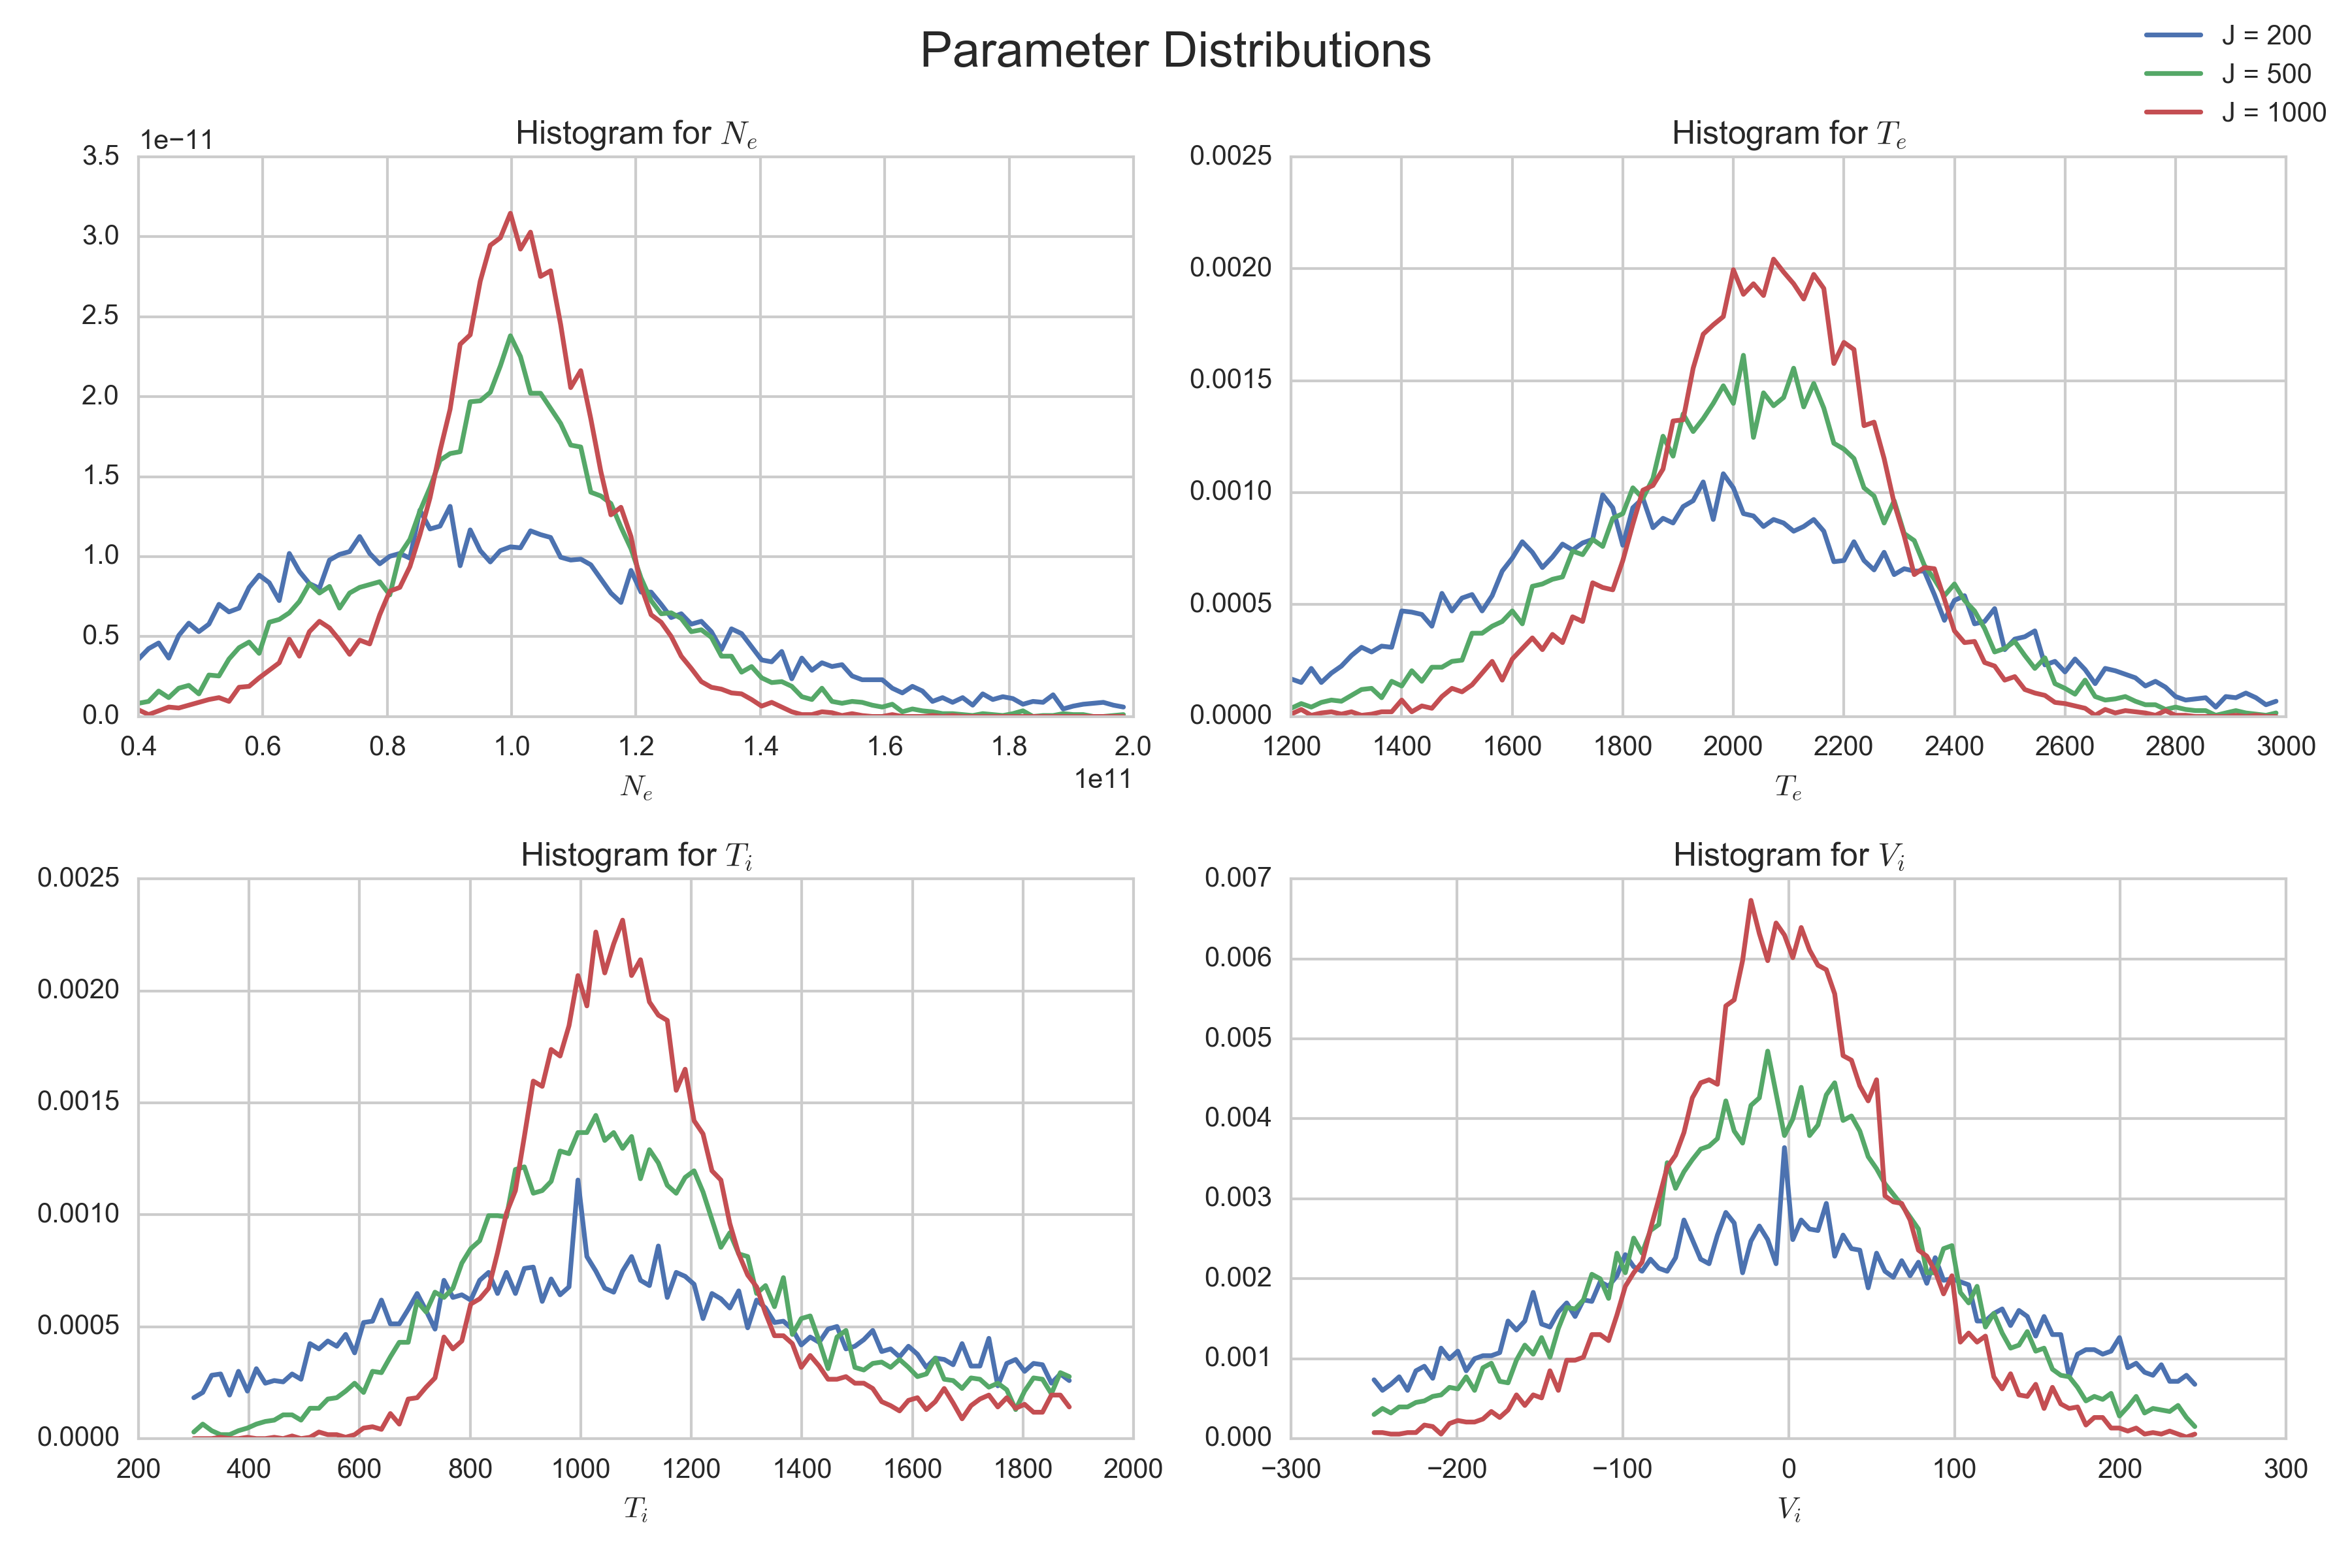
\includegraphics[width=5in]{datahist}
\caption{Normalized histograms of fitted plasma measurements from cases with 200, 500 and 1000 pulses integrated. These are estimates of probability density functions for each of the plasma parameters measurements given the values in Table \ref{tb:param1}.}
\label{fig:statshistall}
\end{figure}

One utility of being able to create a large number of samples of fitted parameters is seen in the error analysis. ISR measurements need to have estimates of the errors, and accuracy of the estimates of these errors can be explored using STISRS. Using case seen in Figure \ref{fig:statshistall} with 1000 pulses we can compare with the actual distribution of parameter values. Figure \ref{fig:statshistsingle} shows gives a comparison of these two different models using, one using the sample variance calculated from each parameter and the average estimate of the error, as the variance and average value for the mean. This example shows that the parameter distributions are well represented by a Gaussian function but that the error estimated from the fit may not give a completely accurate representation of variance of these parameters. 

\begin{figure}[!t]
\centering
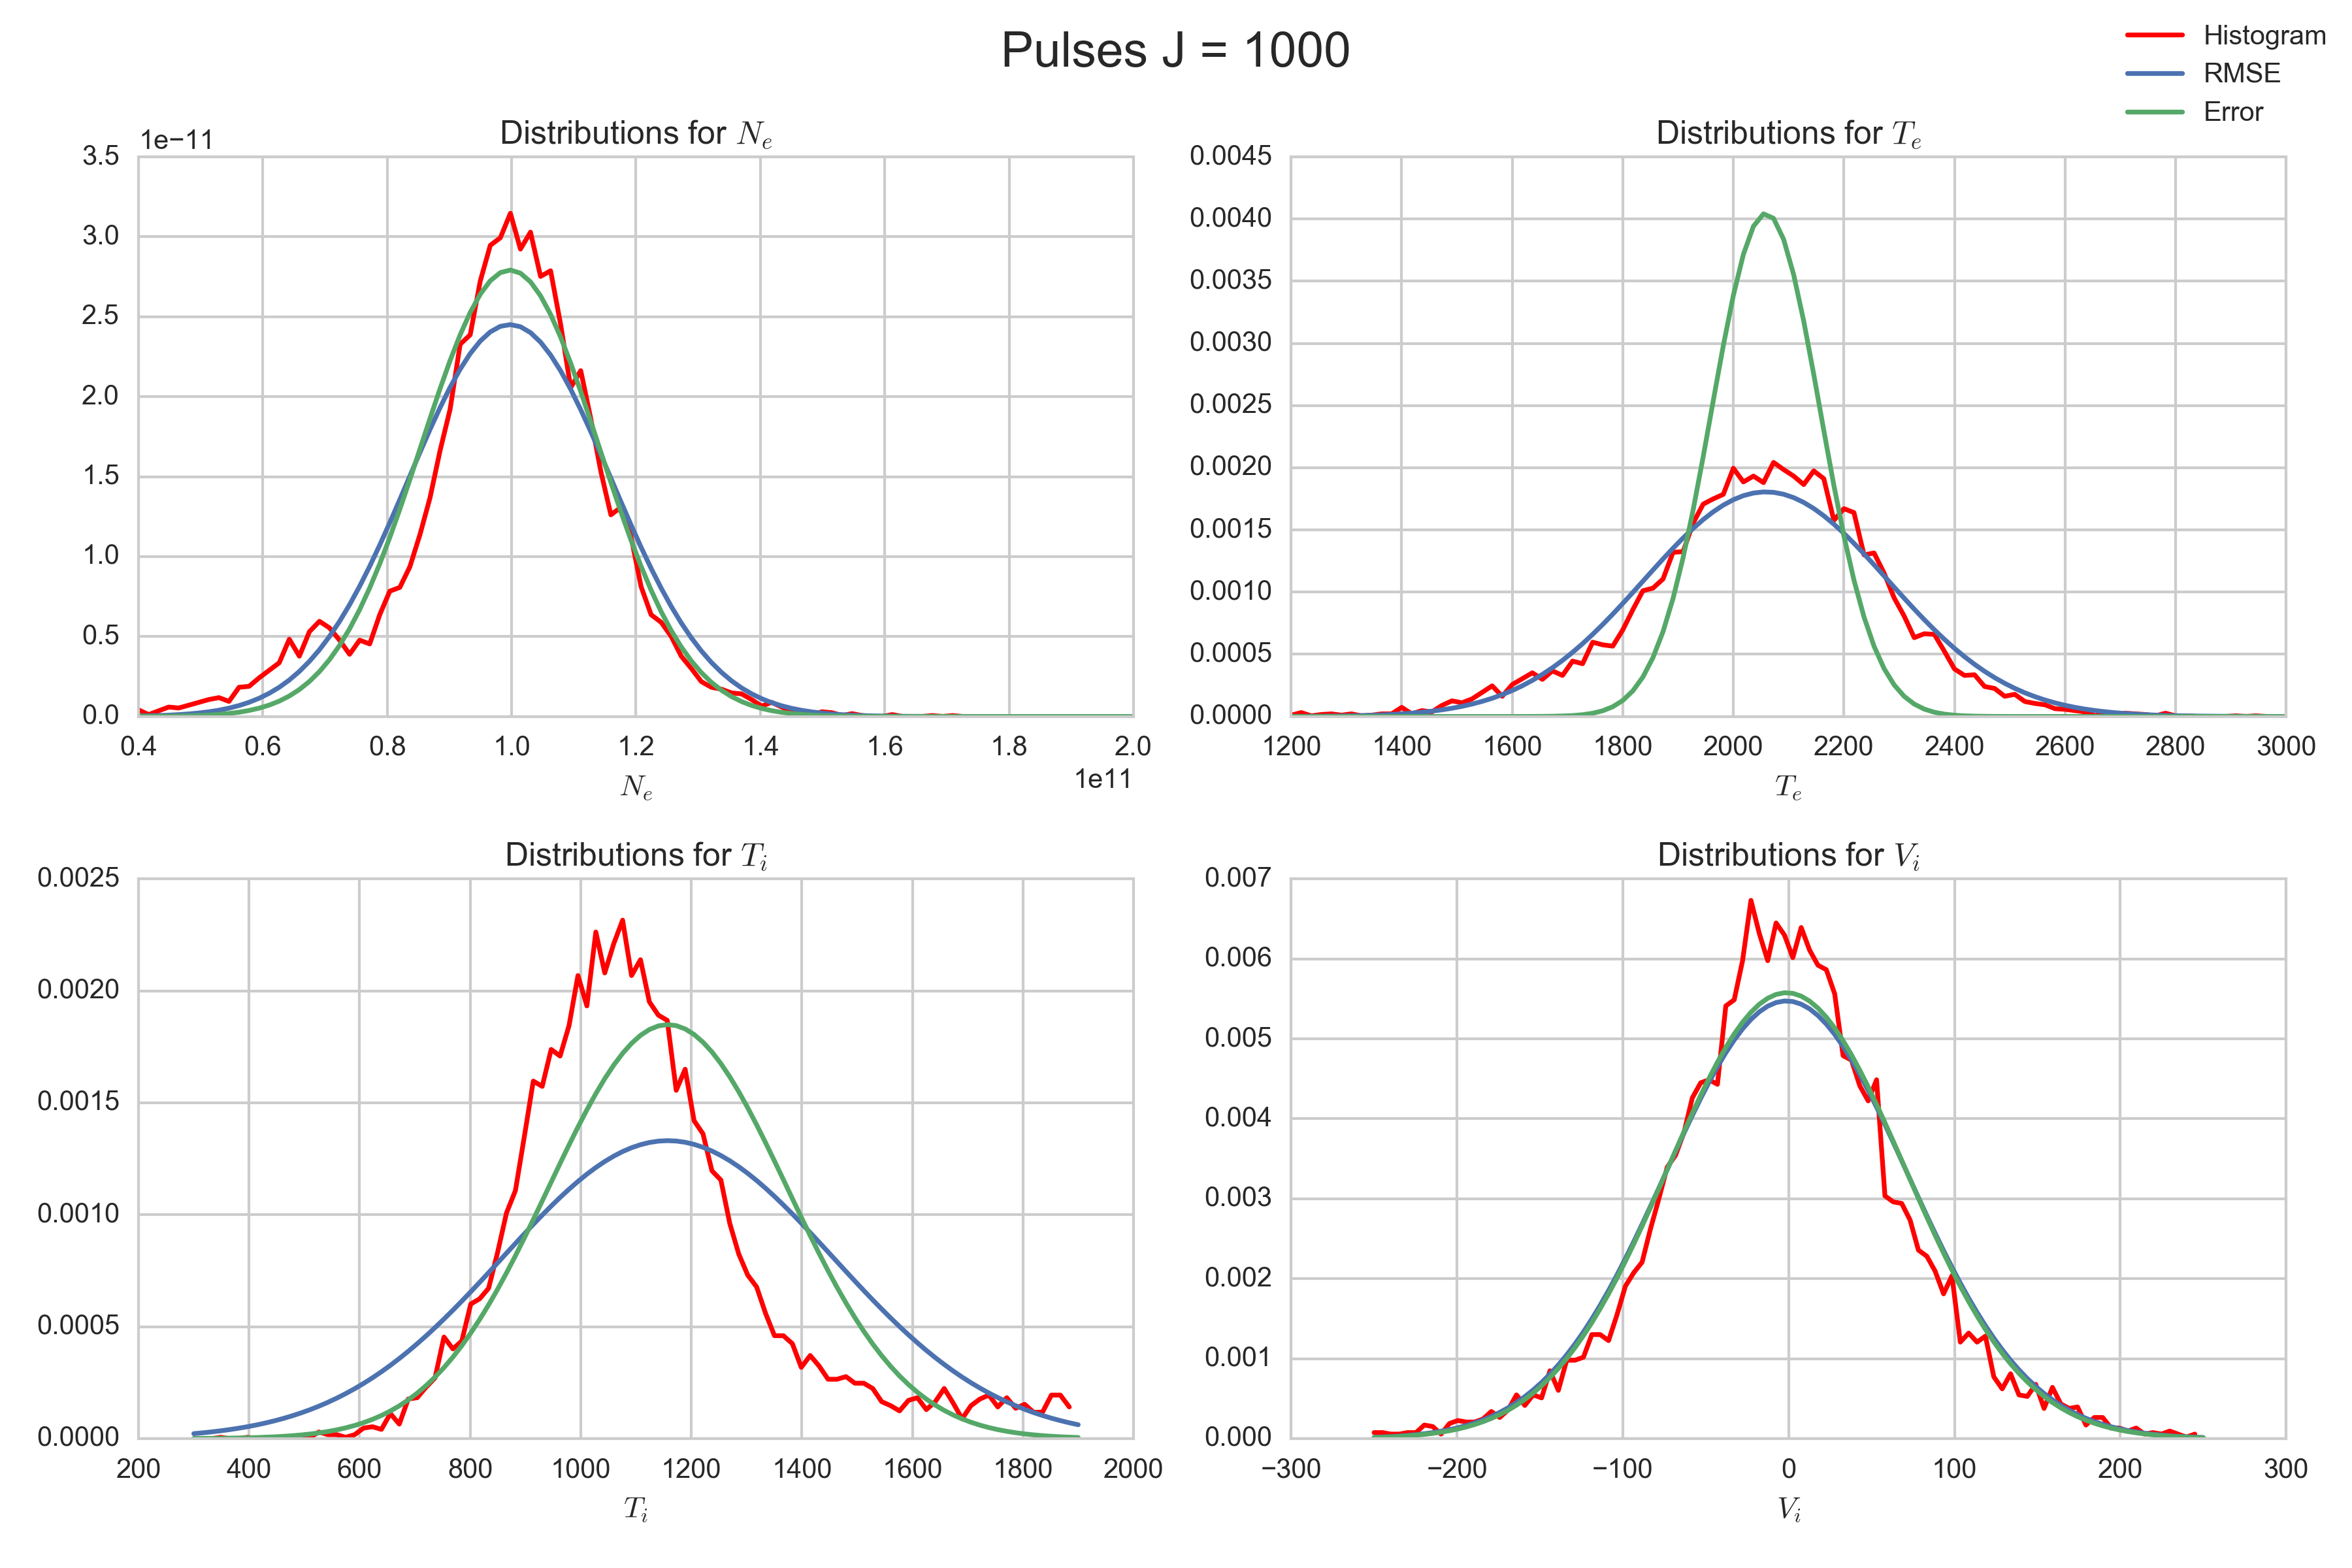
\includegraphics[width=5in]{histsingle}
\caption{Distributions of fitted plasma measurements from cases with 1000 pulses integrated. The red curve shows the actual distribution derived from a histogram of 4600 measurements. The blue curve is a Normal distribution using the MSE from the measurements as the variance and the average parameter value as the mean.  The green curve is a Normal distribution using the average estimate of error squared that comes with the parameter measurement as the variance and the average parameter value as the mean.}
\label{fig:statshistsingle}
\end{figure}


STISRS can useful for identifying situations where assumptions in the parameter fitting break down. For example, a number of studies have explored the case where ISR parameter measurements and spectra show evidence of non-Maxwellian plasma behavior \citep[see, e.g.,][for AMISR examples]{Akbari:2012dz,Akbari:2015fv}. Future studies using the simulator could help create a training set that can be used with a pattern recognition algorithm to identify cases where normal fitting procedures may be incorrect.

\subsection{Electron Density Measurement}
An important aspect of experiment design is determining the observability of plasma phenomena with ISR. The simulator can be used to help understand the trade space accompanying a given experimental configuration. With this in mind, we use a simple two dimensional spatial field of ionospheric parameters as an illustrative case study. An all-O$^+$ ionosphere is created with a background electron density that follows a Chapman function with $1\times10^{11}$ m$^{-3}$ as the peak value and a constant electron and ion temperatures of 2000 $^\circ$K and 1500 $^\circ$K respectively. The background ionosphere is depicted in Figure \ref{fig:background1}.

\begin{figure}[!t]
\centering
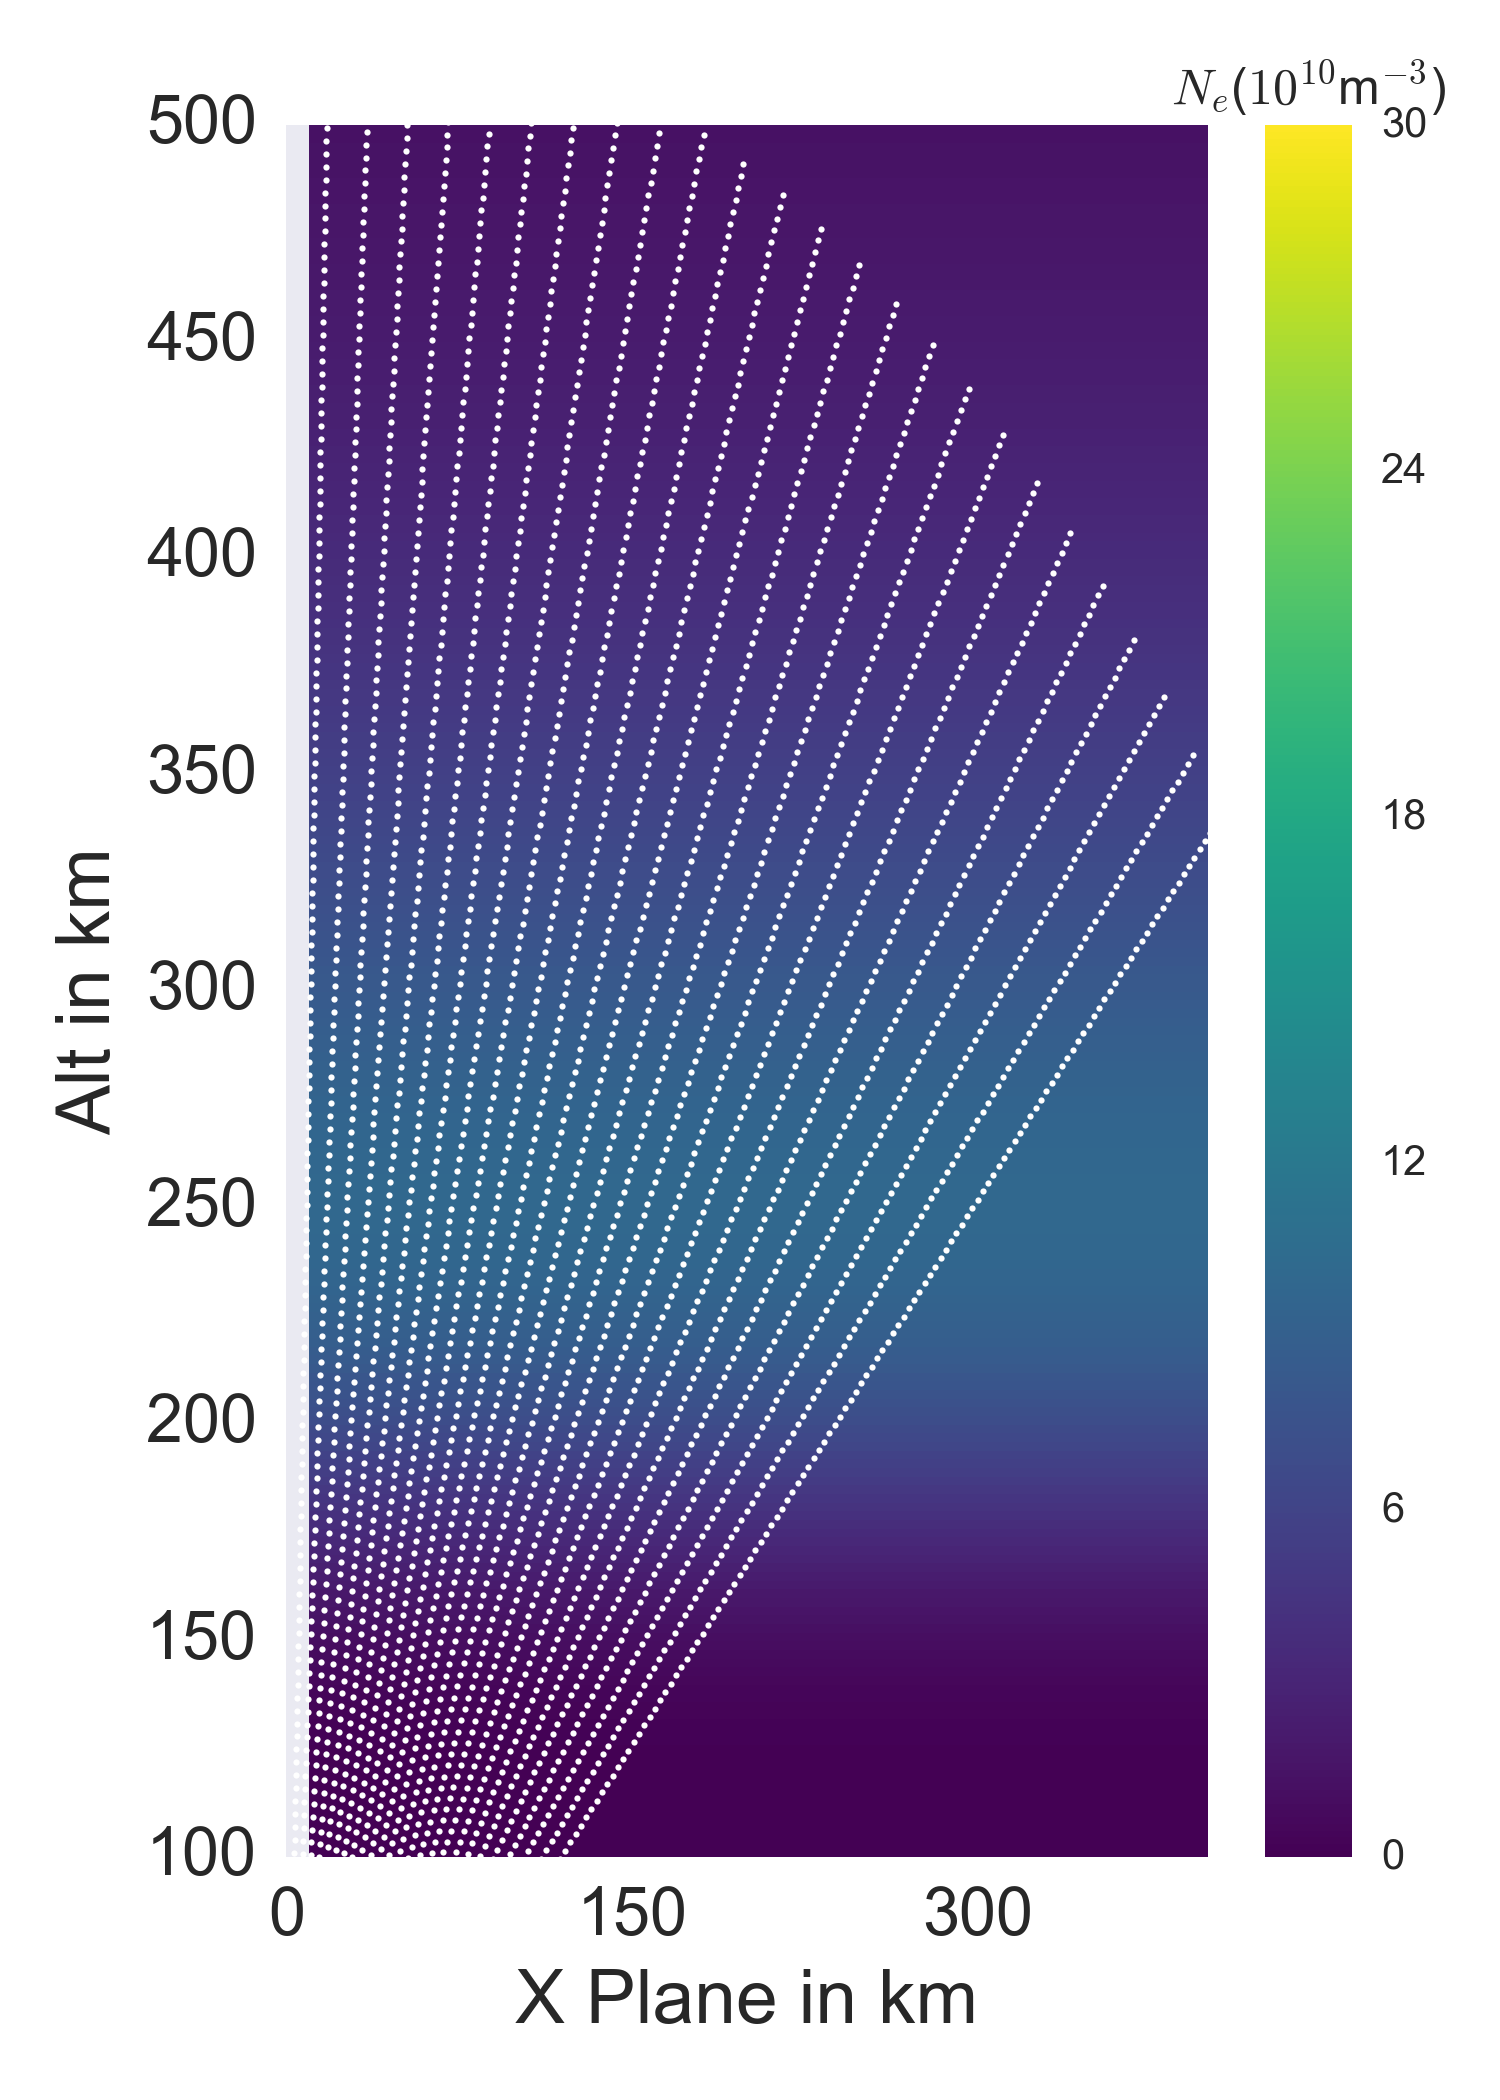
\includegraphics[width=4in]{backgroundandsamp}
\caption{Contour of background $N_e$ for simulations and the spatial sampling pattern}
% JOHN:  you don't need both of these panels, just the one on the right along with the colorbar.   Also, you should reduce the number of labels on colorbar, increase the font, and absorb exponent into units (which are not given).  Also there is no indication of what scalar is being plotted.   Typically you would write parameter/units above the colorbar:   $N_e (10^{10}$m$^{-3})$.   This comment goes for other plots too.
\label{fig:background1}
\end{figure}

%For these simulations we want to show how ambiguities could arise when trying to image just simple electron density enhancements with the beam pattern shown in the right panel of Figure \ref{fig:background1},
We first explore how a thin stationary density enhancement is resolved with the radar beam pattern shown in Figure \ref{fig:background1}, where each dot is a range gate in one of the 25 beams used. In Figure~\ref{fig:stationaryall}a, a thin density enhancement 2 km in width and 5 times the background is placed in the radar field of view. The enhancement is at the resolution limit of the original Cartesian grid, a delta function in the x direction.  The results of a single realization of our simulation 
%JOHN:  I don't know what "results of a single realization of our simulation" means here.  Is this different than "results of our simulation"?
are seen in Figure \ref{fig:stationaryall}b and c using 15 and 60 second integration times, corresponding to 60 and 240 pulses per position, respectively. The different integration times show that although the enhancement is blurred the variance of the measurement impacts the quality of the reconstruction because of the inherent noise-like nature of of the signal. The expected errors for both of the reconstructions are shown in \ref{fig:errorstationaryall}. As expected the estimated errors show the uncertainties for the case with less pulses to be larger. 
%JOHN:  I've tried to fix figure referencing in the above since it didn't mesh with what you had.   Also, how are you deriving density, is it just range corrected power here, or full spectrum fitting?  

Because we know the input parameters, we can do a quick comparison using the root mean squared error (RMSE) for each case. If we comparing the RMSE between the 15 and 60 second integration cases we find that the ratio between the two is approximately 5.4. The expect RMSE ratio between the two should be about 2 because the variance of the ACFs scales as $1/\sqrt{J}$, where $J$ is the number of pulses. If we instead use a median instead of a mean operator in the error calculation, this ratio becomes 1.55, which is some what more in line with what is expected.

\begin{figure}[!t]
\centering
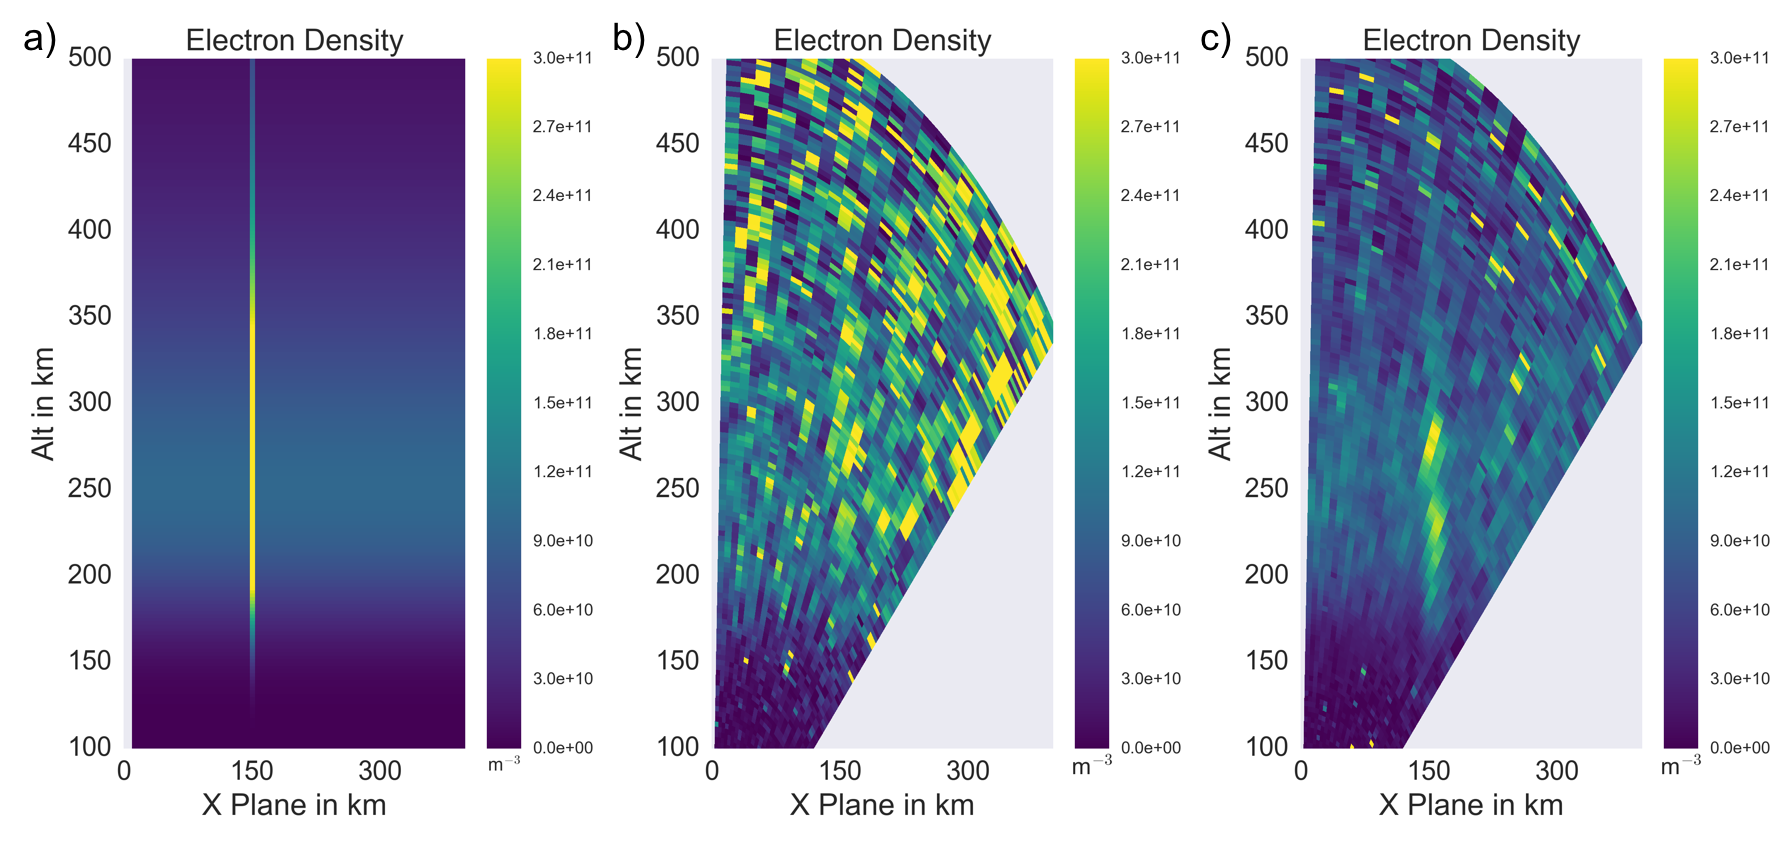
\includegraphics[width=6in]{stationary}
\caption{Results of stationary enhancement simulation. a) Input $N_e$. b) Output of simulator with 15 second integration. c) Output of simulator with 60 second integration.}
\label{fig:stationaryall}
\end{figure}

\begin{figure}[!t]
\centering
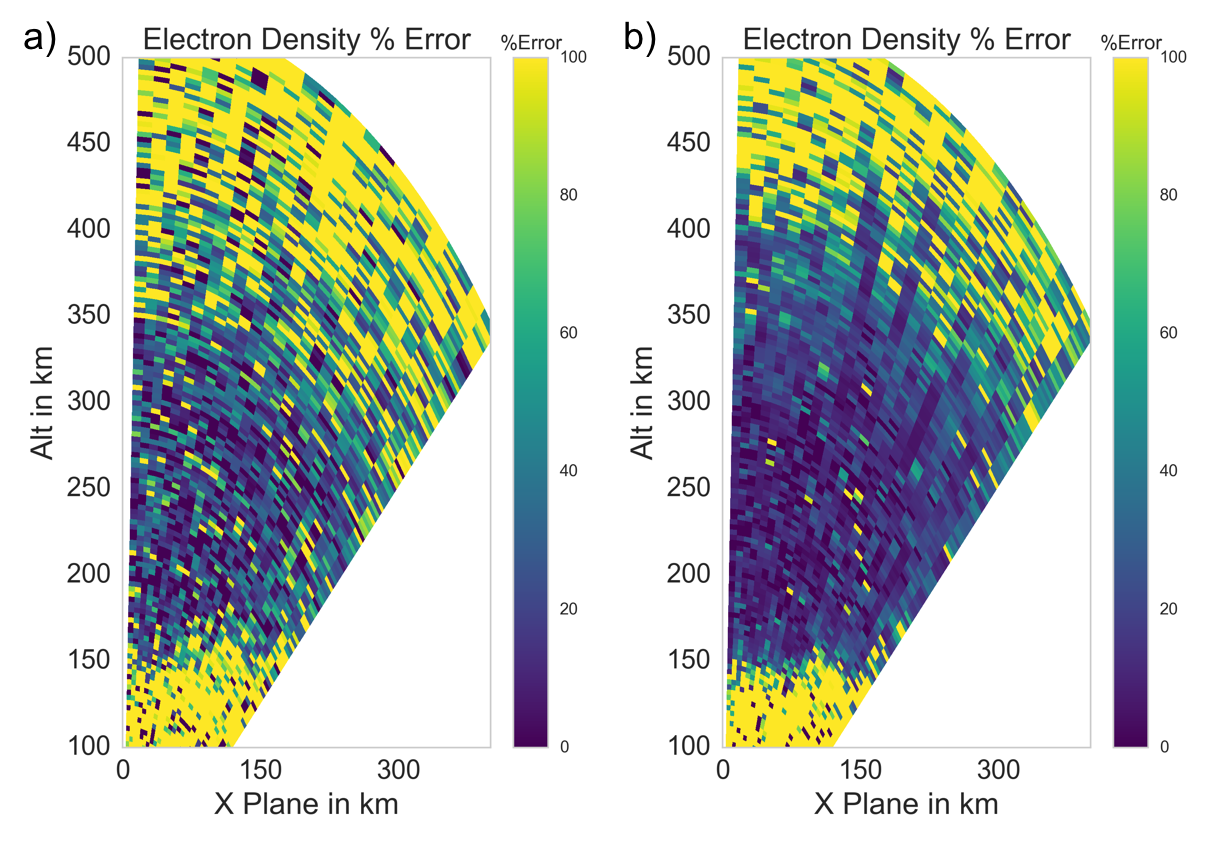
\includegraphics[width=4in]{Errorstationary}
\caption{Standard deviations from Figure \ref{fig:stationaryall}. a)  Estimate from fit for 15 second integration example. b) Estimate from fit for 60 second integration example.}
\label{fig:errorstationaryall}
\end{figure}

The blurring effect seen in this case study is not constant throughout the space due to the way the radar samples the space. This is illustrated in Figures \ref{fig:moving10mins} and \ref{fig:moving14mins}, where as the enhancement moves through the scene, its apparent size is affected by the orientation of the radar beams. As the enhancement becomes parallel to the radar beams then its morphology in the reconstruction becomes smaller along the x-axis, as the range ambiguity is much larger than the cross range ambiguity. (To see the input and output electron density change with time, the reader is referred to Movies S1 and S2.)

\begin{figure}[!t]
\centering
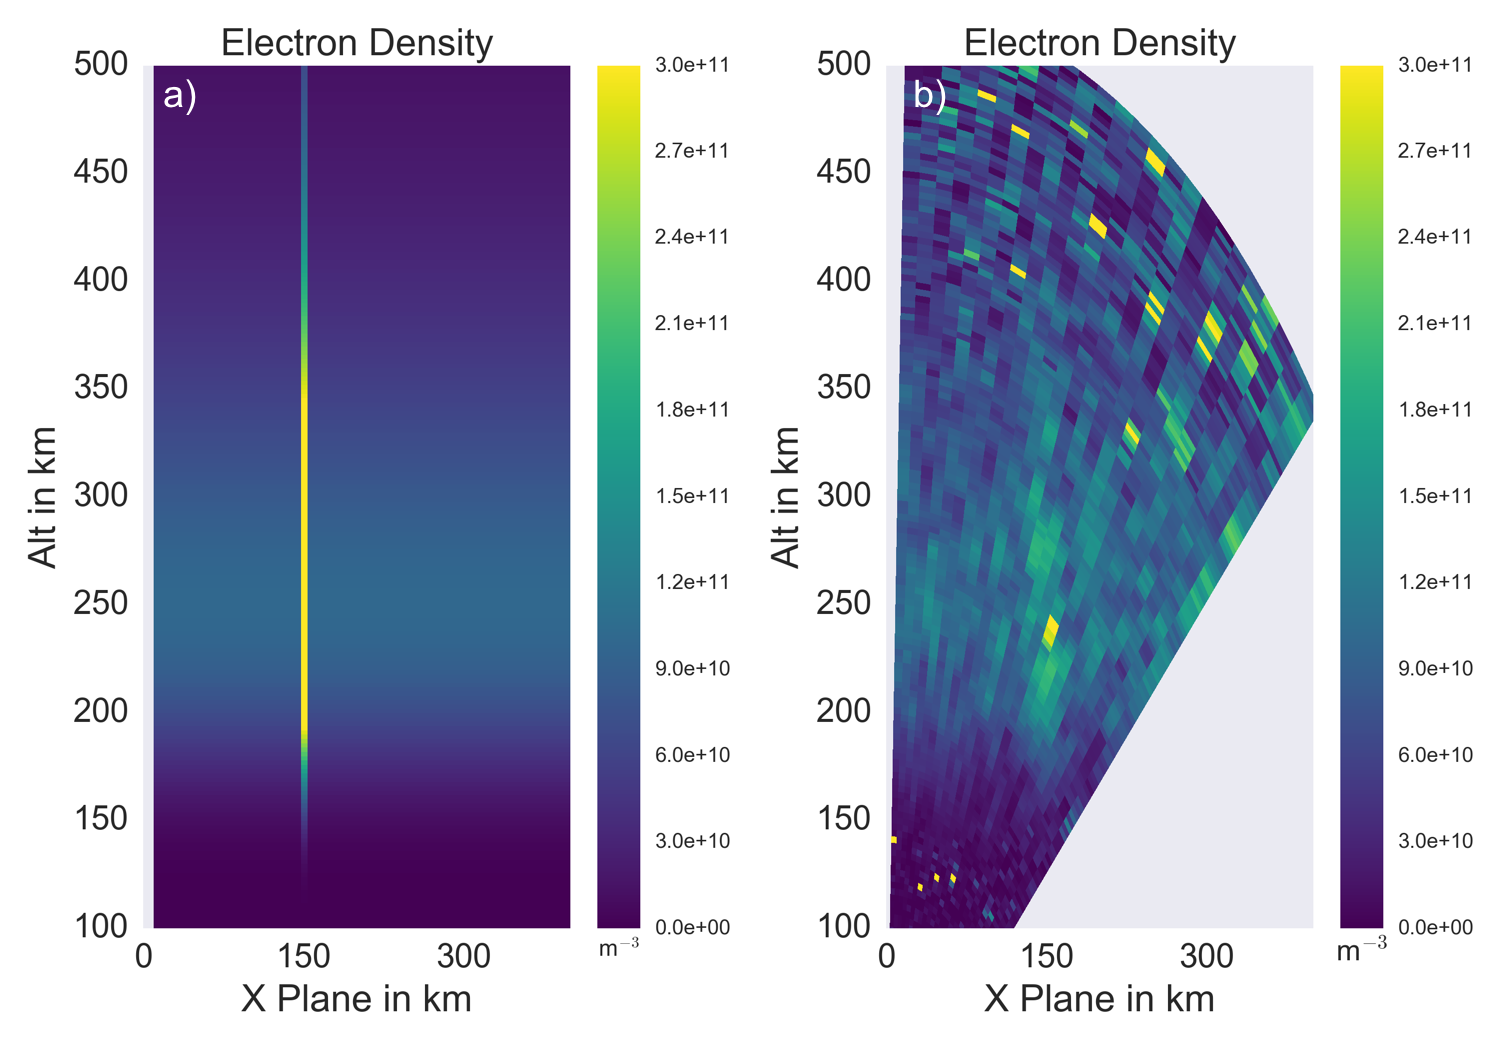
\includegraphics[width=6in]{moving6mins}
\caption{Results of moving enhancement simulation at 600 seconds. a) Input $N_e$. b) Output of simulator with 60 second integration. c) Estimated errors from fit.}
\label{fig:moving10mins}
\end{figure}


\begin{figure}[!t]
\centering
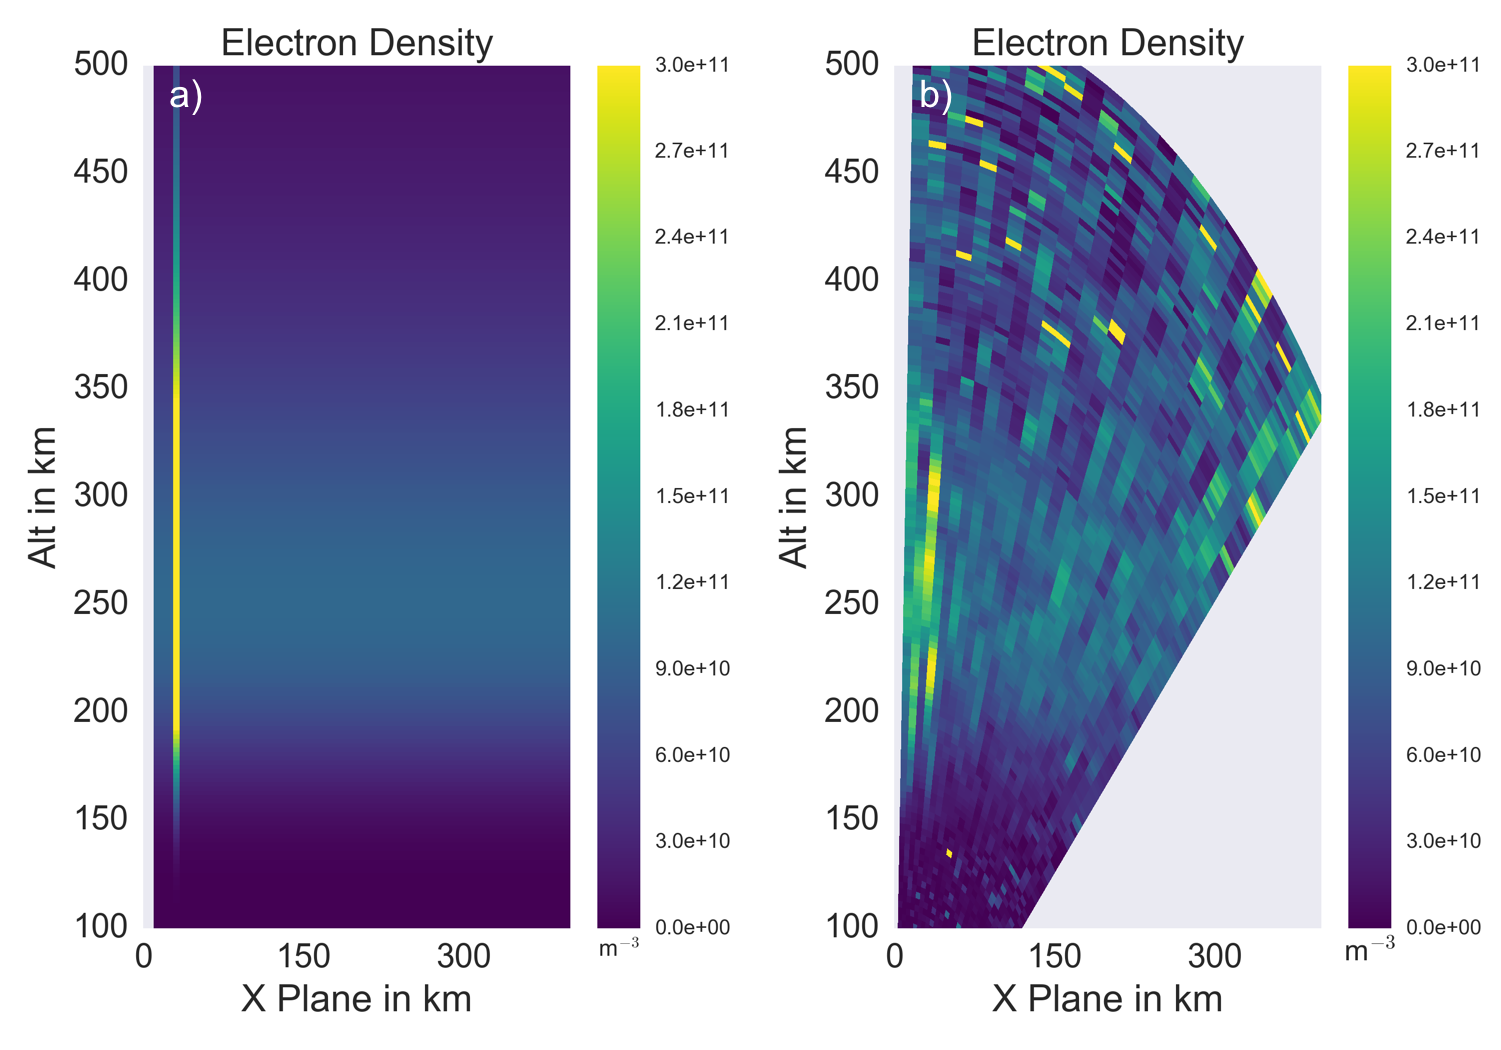
\includegraphics[width=6in]{moving14mins}
\caption{Results of moving enhancement simulation at 840 seconds. a) Input $N_e$. b) Output of simulator with 60 second integration. c) Estimated errors from fit.}
\label{fig:moving14mins}
\end{figure}

This change in the shape of the enhancement can give the impression that its morphology has evolved as it was moving through the field of view of the radar. This could lead to an incorrect interpretation of the physical process taking place, and issue raised by \citet{Dahlgren:2012dq}.   Thus one must be careful when analyzing these sorts of reconstructions.

Lastly, for this type of simulation, we show an example to demonstrate the situation where a set of two different input parameters can yield qualitatively similar results. For these cases we create electron density enhancements similar in size as what is seen in \citet{Semeter:2005fo} from a poleward boundary intensification event. The sizes of these enhancement are 10 km width and 18 km width. The enhancement in the 10 km width example is 6 times higher than the background while the 18 km width enhancement is 3 times higher than the background.

The input electron density, the fitted electron density and the expected error for the 10 km enhancement can be seen in Figure \ref{fig:moving10all}. The same images for the 18 km wide case can be seen in Figure \ref{fig:moving18all}. Both cases show that electron density enhancements are well above the expected errors. The fitted electron density for 10 km enhancement the 18 km enhancement show nearly identical results. This simple example demonstrates the possibility to create a non-unique solution in ISR. But it also shows a utility for STISRS in that it can be used to determine if an experiment set up will lead to ambiguous results between two different sets of phenomena. (For the full input electron density changing with time for the 10 km example with time see Movie S3 and for the fitted data S4. The 18 km case can be seen in Movies S5 and S6 for input and fitted parameters respectively.)

\begin{figure}[!t]
\centering
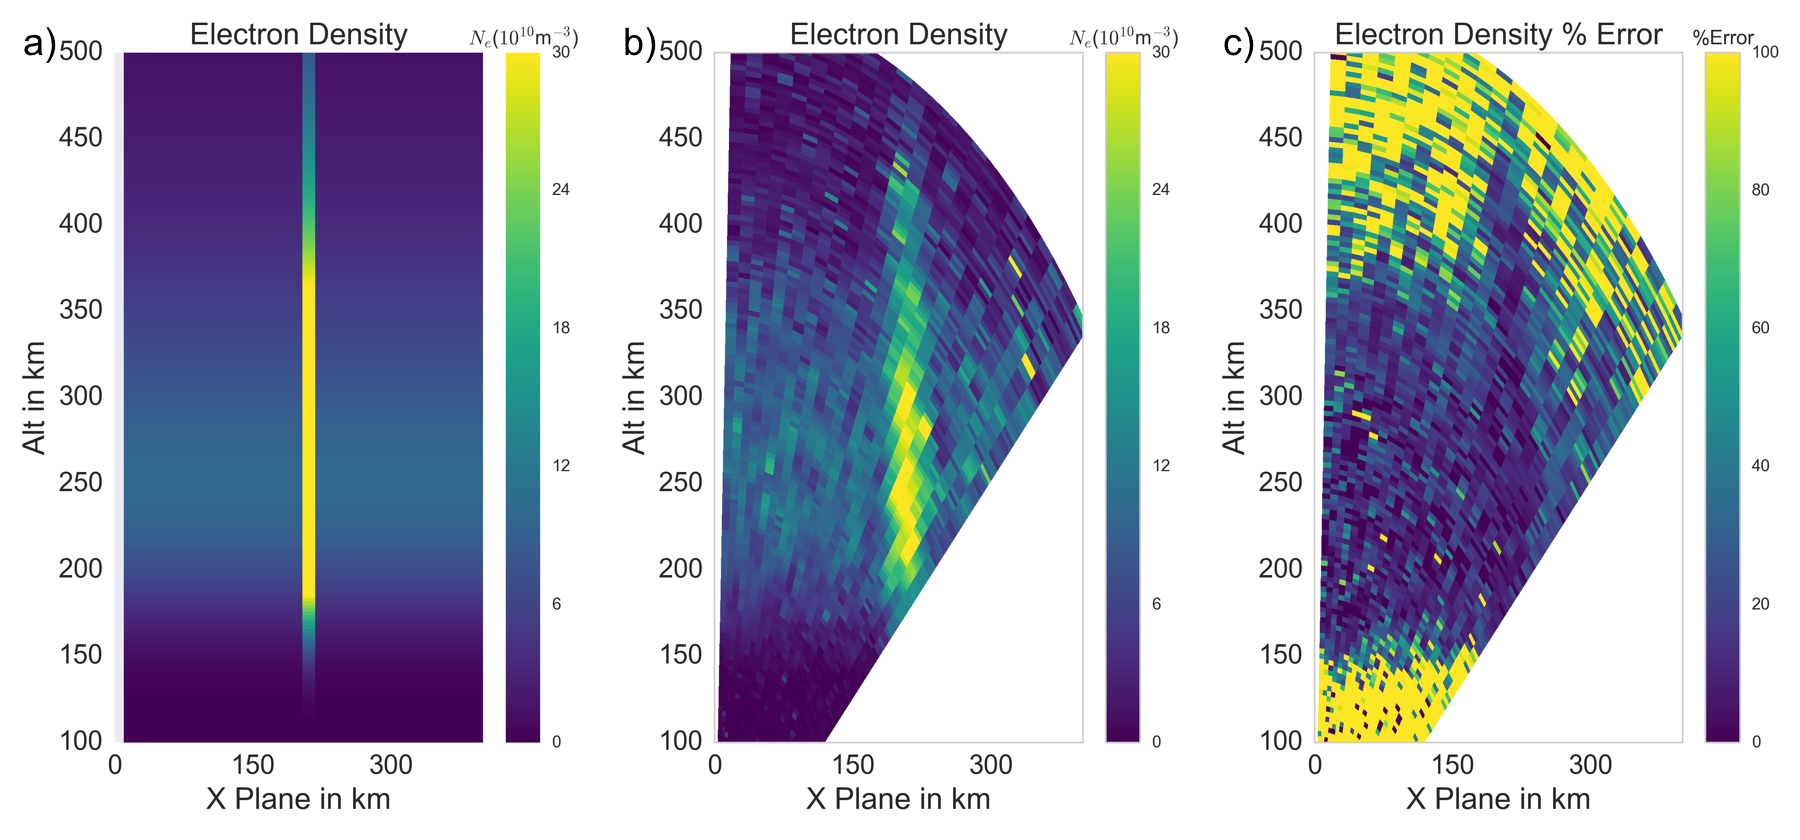
\includegraphics[width=6in]{moving10kminouterr}
\caption{10 km wide enhancement moving simulation at 480 seconds. a) Input $N_e$. a)  b) Fitted $N_e$ with 60 second integration. c) Estimated error from fit.}
\label{fig:moving10all}
\end{figure}

\begin{figure}[!t]
\centering
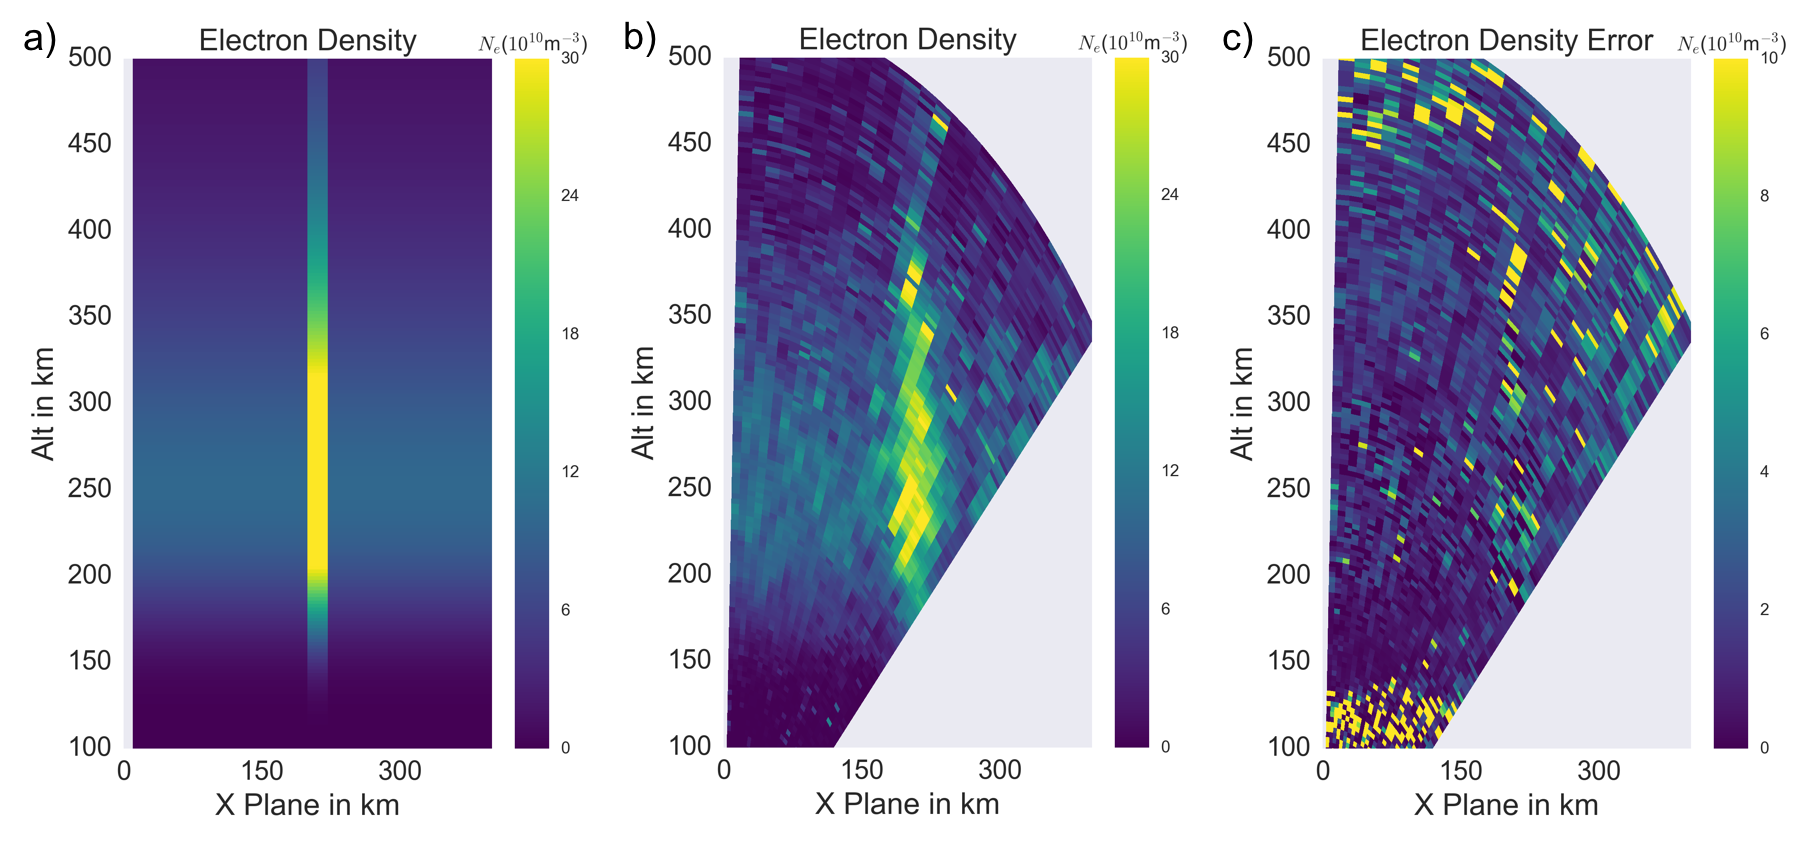
\includegraphics[width=6in]{moving18kminouterr}
\caption{18 km wide enhancement moving simulation at 480 seconds. a) Input $N_e$. a)  b) Fitted $N_e$ with 60 second integration. c) Estimated error from fit.}
\label{fig:moving18all}
\end{figure}

\subsection{Full Parameter Experiment}
\label{sec:fullparam}
Finally, plasma parameters derived from the multi-fluid model developed by \cite{semeter:plasmatransport2012} are used to drive STISRS. The specific model run was originally used by \cite{Perry:2015jf} to assist in interpreting measurements from the Resolute Bay Incoherent Scatter Radar (RISR). Images of the modeled plasma parameters are shown in Figures \ref{fig:plparamst0} and \ref{fig:plparamst60}. The enhancements in electron density, electron temperature, and ion temperature represent the self-consistent regional response of the ionosphere to an field-aligned current system with amplitude .875 $\mu$A/m$^2$ that moves with respect to the radar with a velocity of 200 m/s.   We thus have a physically self-consistent evolution of ionospheric state parameters in space and time.   A reasonable objective for a multi-beam ISR experiment could be to validate such a model prediction.  STISRS can be used to assess the observability of this dynamic and establish confidence intervals on the results.  

\begin{figure}[!t]
\centering
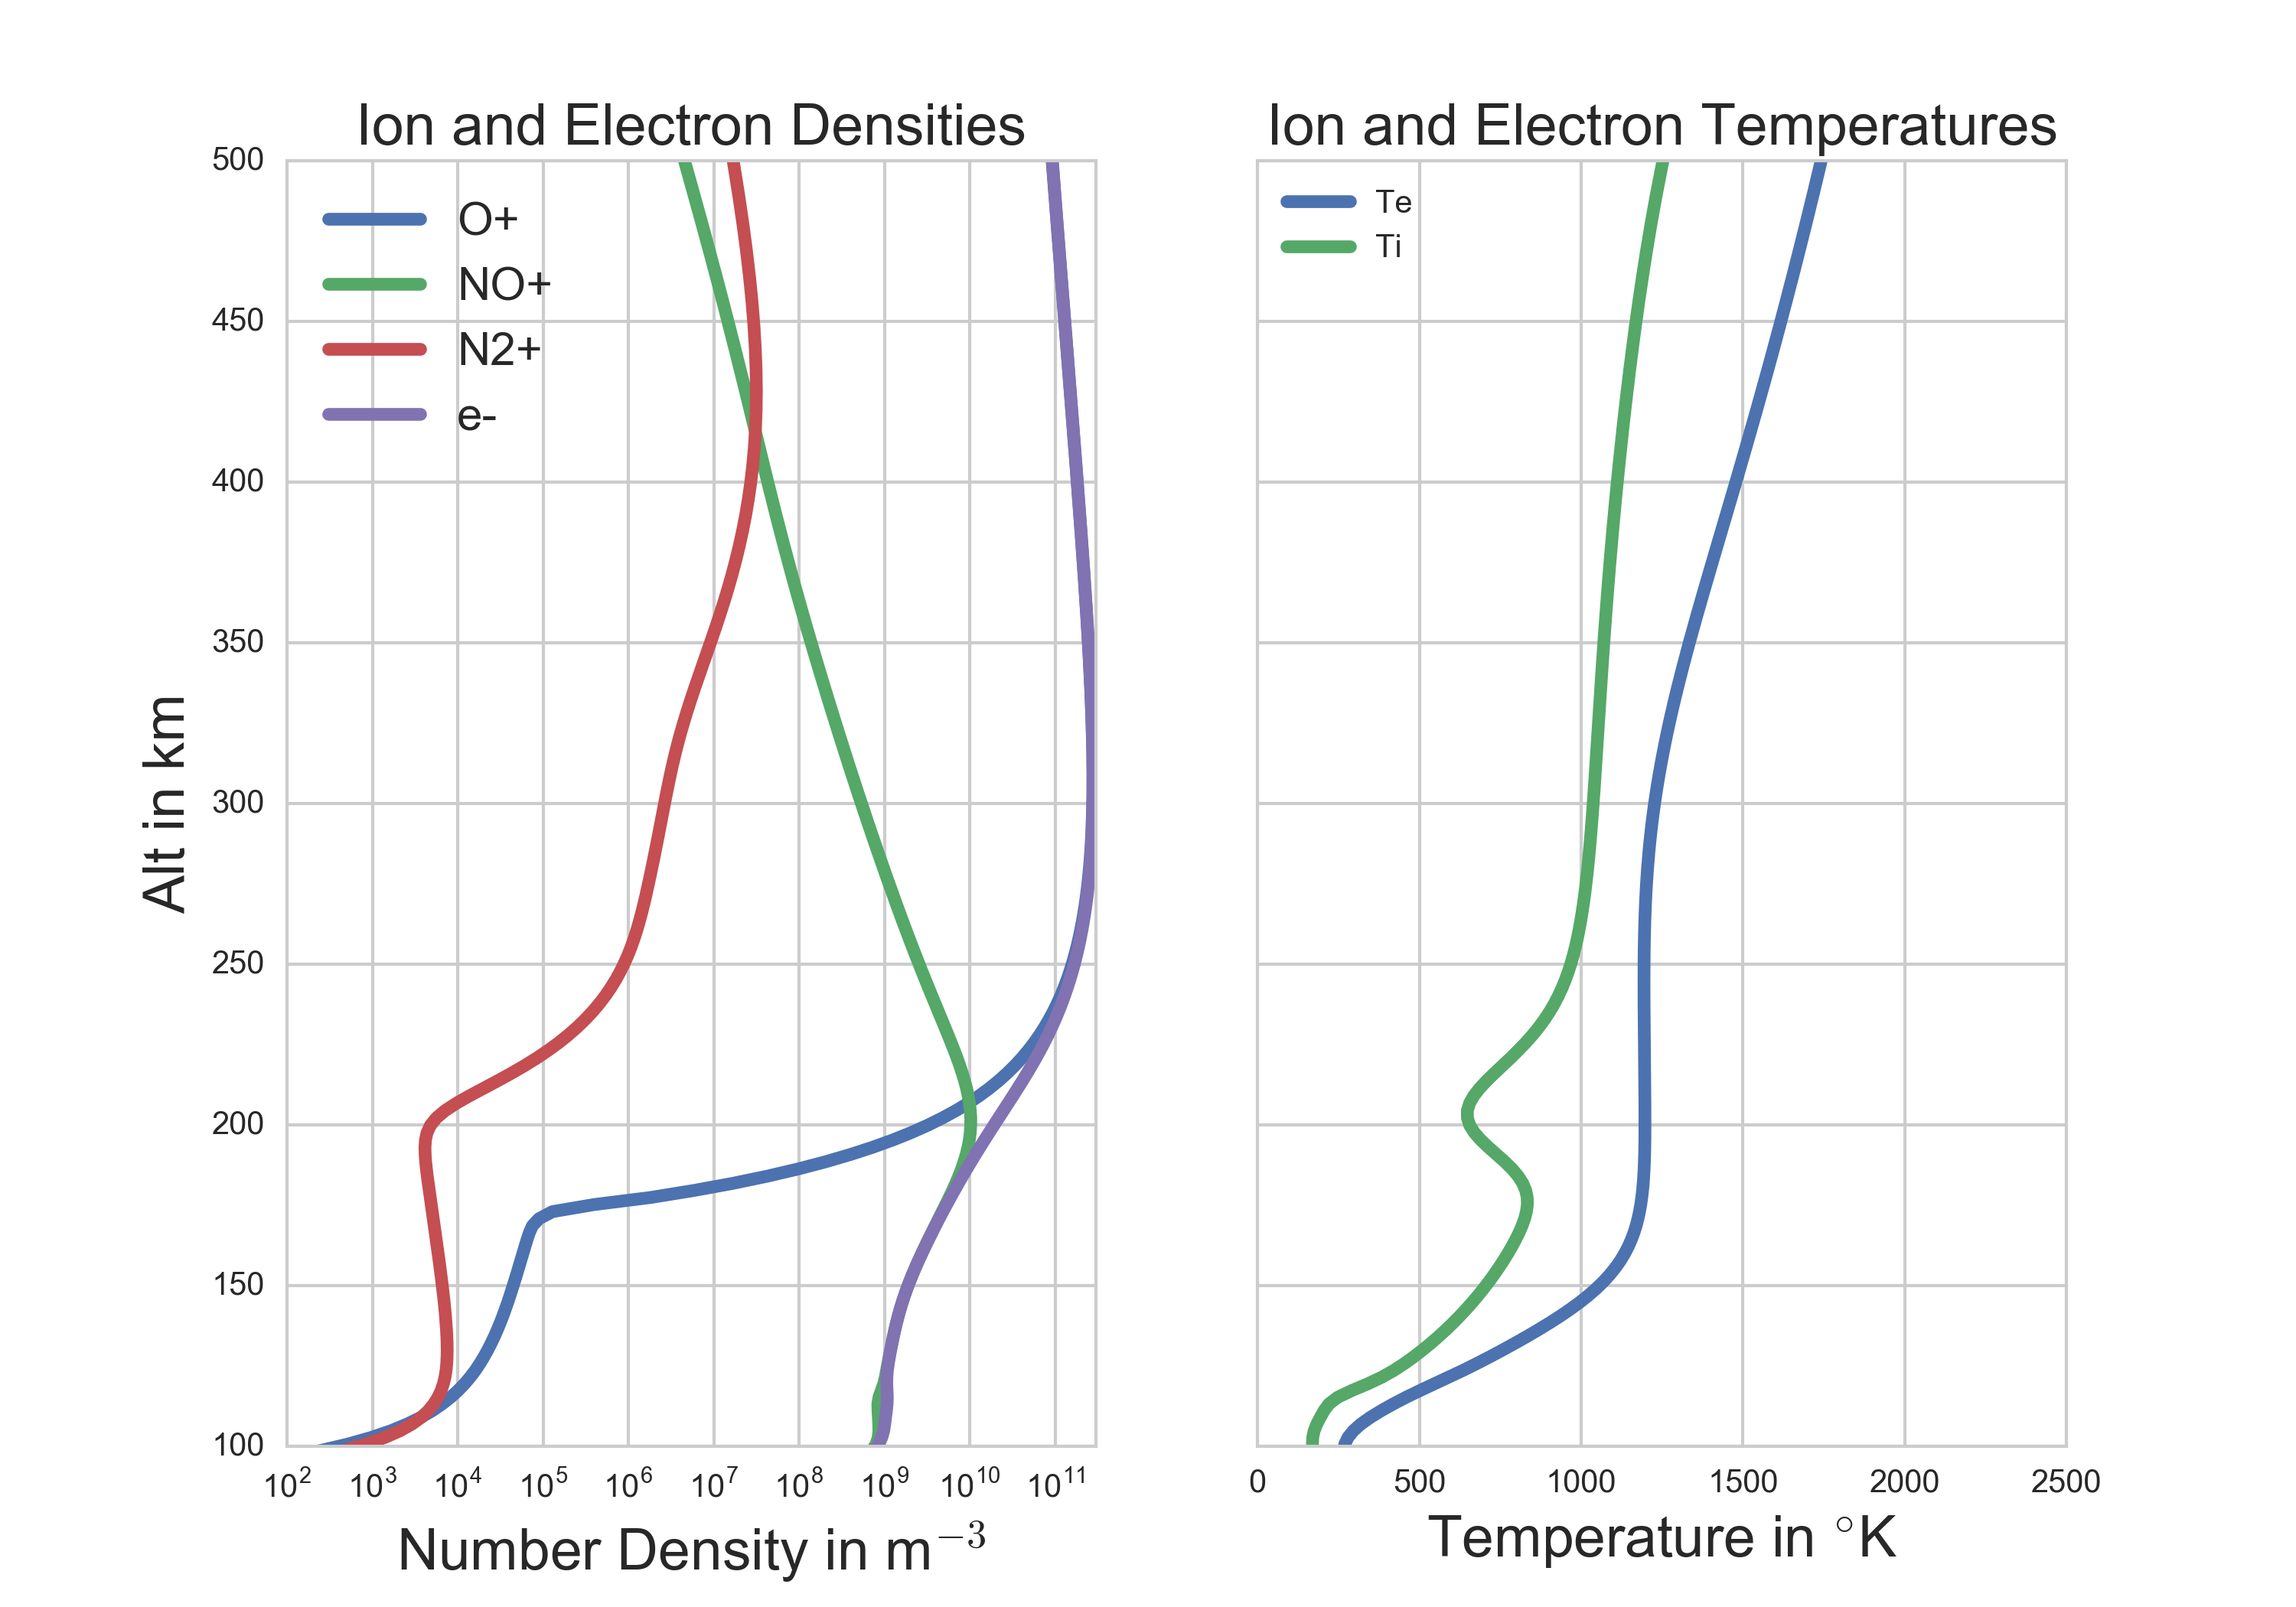
\includegraphics[width=6in]{backgroundallparams}
\caption{Background ionospheric parameters ($N_e$, $T_e$, $T_i$) along with number density of ion species, used for simulations.}
\label{fig:plparamst0}
\end{figure}

\begin{figure}[!t]
\centering
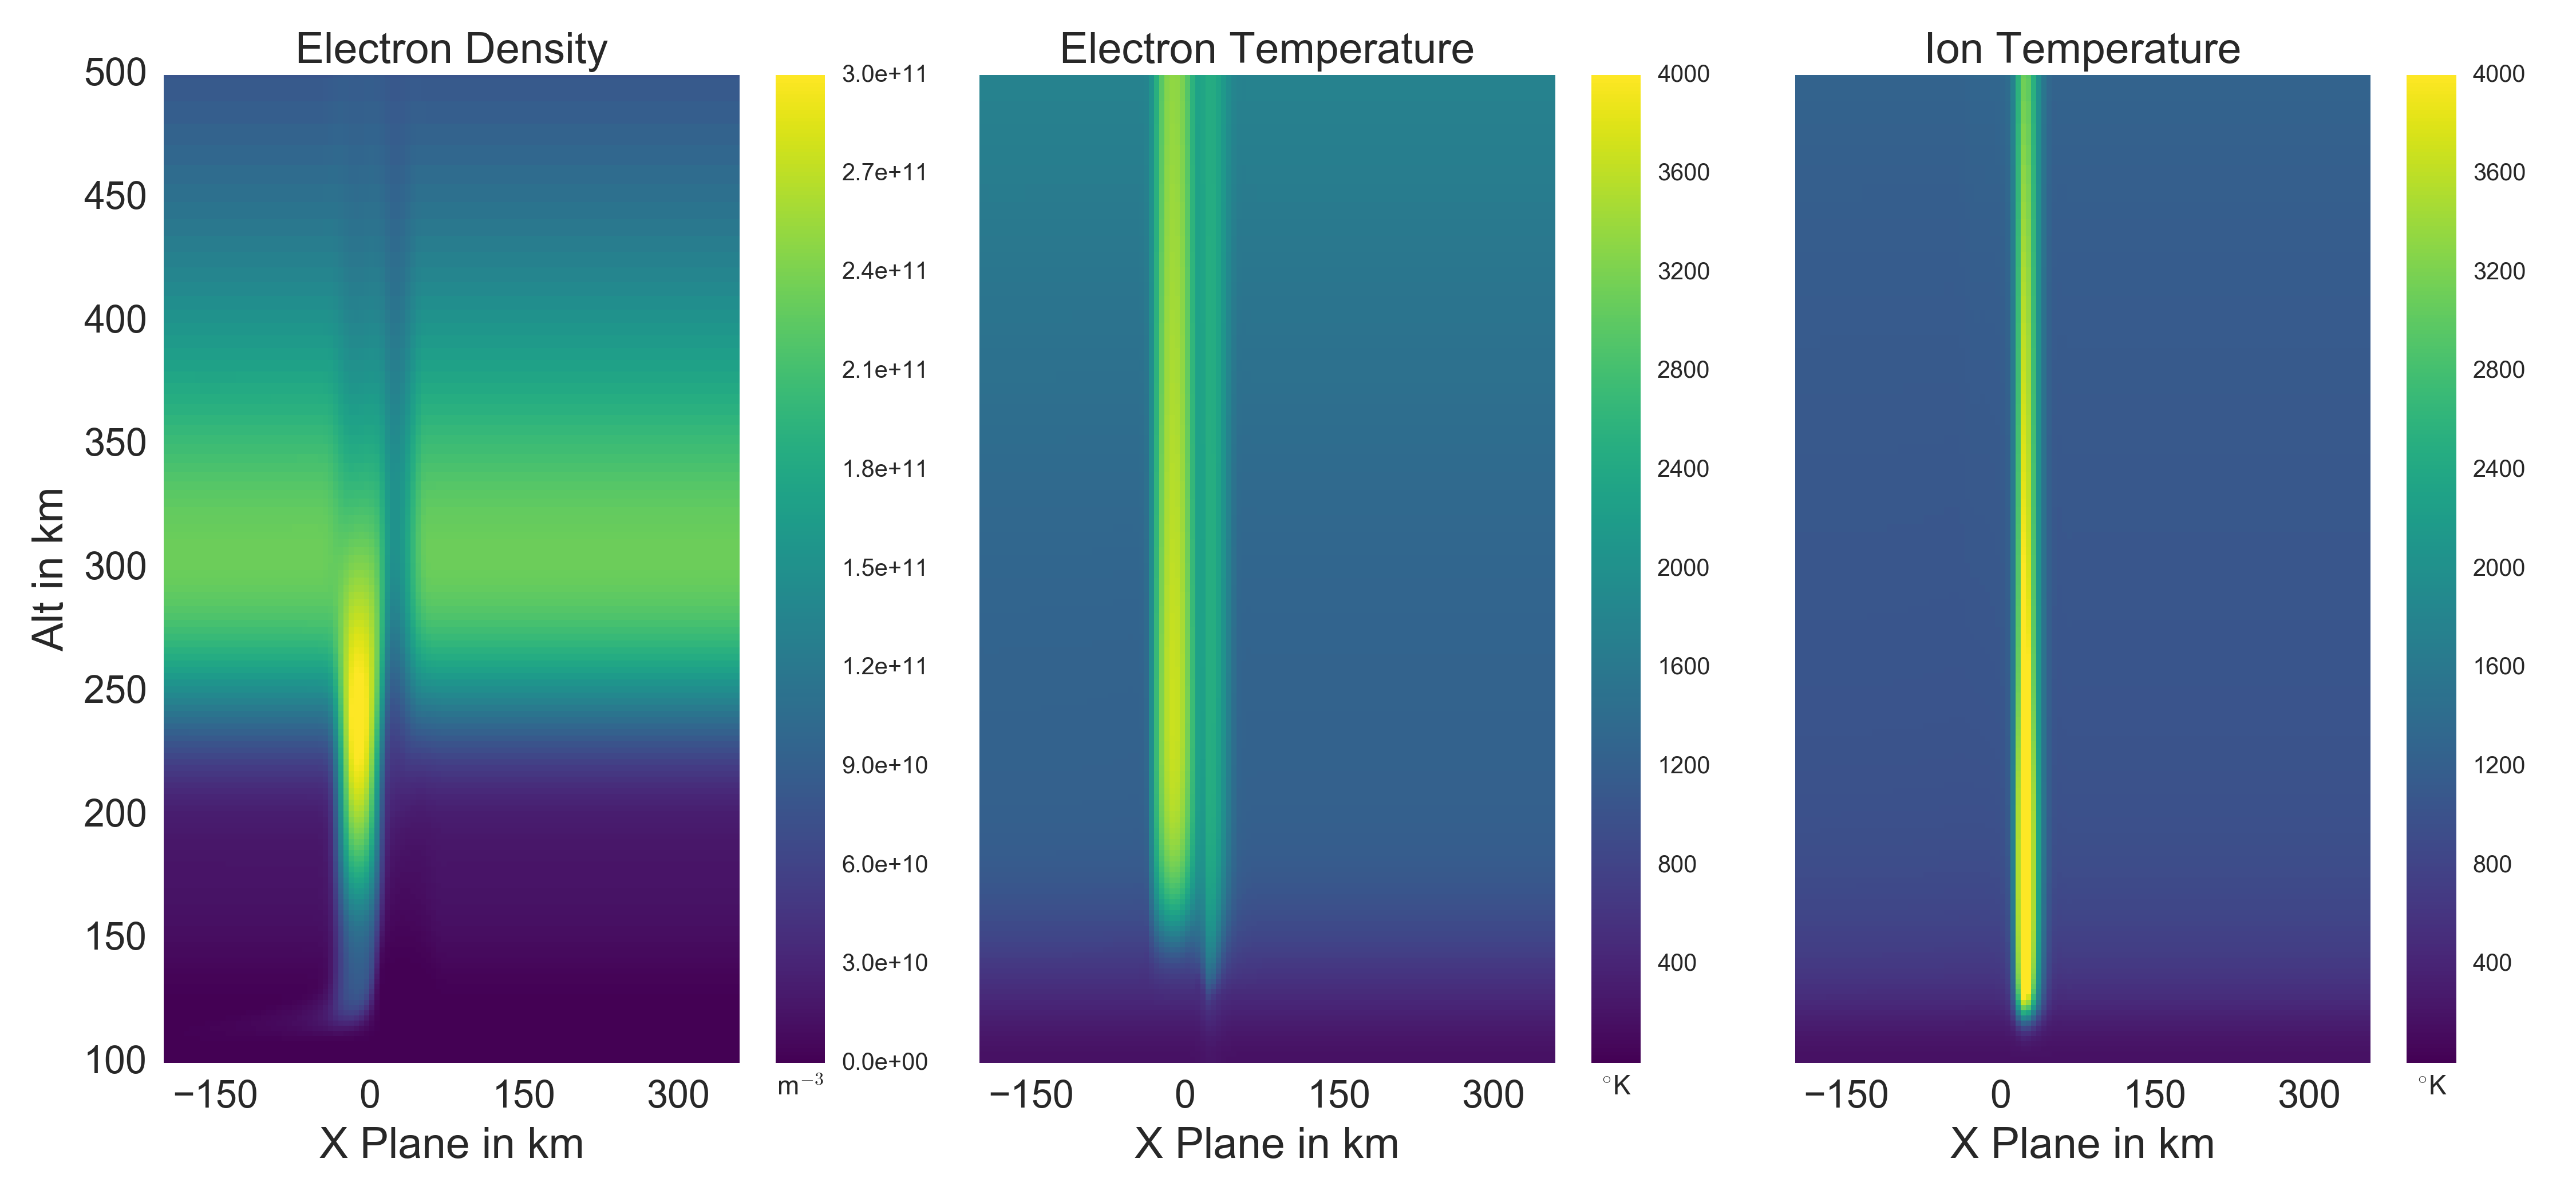
\includegraphics[width=6in]{0960_15_int}
\caption{Perturbations to Figure \ref{fig:plparamst0} due to an imposed current system of .875 $\mu$A/m$^2$ at $t=960$ s, auroral arc.}
\label{fig:plparamst60}
\end{figure}

Using a beam pattern similar to the one seen in the right panel of Figure \ref{fig:background1}, we use STISRS to explore how an electronically scanned ISR may reconstruct this dynamic.  For the purposes of illustration, we use the contrived case where the radar spatial beam pattern is defined to be in the plane of convection.  It is also assumed that the ratios between ion species are known. This is a common practice in ISR fitting, as allowing the ratios to be free parameters can allow for non-unique solutions depending on the ion species that are present. If the fixed, apriori assumed composition ratios between the different ion species are incorrect, this can lead to errors in the final parameter estimates. For the lower F region ionosphere, this generally leads to errors between 150-250 km where the ionosphere changes from NO$^+$ dominated to O$^+$ dominated \citep{Zettergren:2011ej, Blelly:2010gf}. Another aspect from this specific case as the field aligned current passes through this creates an influx of  NO$^+$ in the crossover region for this simulation \citet{Perry:2015jf}.
% JOHN:  I can't figure out what the above sentence fragment is supposed to be.

The output of the STISRS from the parameters can be seen in Figure \ref{fig:fplparamst60} and in Movie S8. The integration is started at $t=960$ s into the simulation with the plasma parameters shown in seen in Figure \ref{fig:plparamst60}. The full set of plasma parameters over time can be seen in Movie S7. For this case, a 60 second integration time is used, which for the 27 beam radar experiment set up gives 255 pulses per position. Lastly the expected errors from the fit can be seen Figure \ref{fig:fplparamst60err}.

We highlight several features in the fitted results. First, the predicted enhancements in electron and ion temperature are clearly observable and well above the expected error. Second, we examine whether the predicted density cavity in the downward field-aligned current region is  detectable.  A deepening and broadening region of plasma evacuation is predicted as a self-consistent response to a confined up-down current pair \citep[e.g.,][]{wright;alfven}.  But it has been unclear whether this prediction can be validated with ISR, since it involves detecting coherent channels of reduced backscatter power embedded within a higher density background. 

The images shown in \ref{fig:fplparamst60} represent the best case scenario for identifying the presence of this cavity since, at this time, the cavity is nearly co-aligned with one of the beams. 
%For the other cases where the beams are not well aligned with the cavity it becomes much more difficult to observe it due to the range ambiguity being larger than the beam width, making the "filling in" of the evacuated electrons more pronounced. 
Using density measurements alone (panel a) the presence of the cavity is visible, but only marginally so as it is blended with the adjacent  enhancement produced by the applied precipitation in the upward current channel.  A similar ambiguity exists with the electron temperature result, which could easily be interpreted as purely an effect of heating from soft precipitation.   However, the ion temperature increase in panel b is decidedly narrower than the electron temperature enhancement, offering a possible observable fingerprint for the presence of a confined up-down current pair.  The simulation result illustrates the efficacy of a collective analysis of all plasma state parameters in evaluating the physical mechanism responsible for an observed dynamic.  This is a common approach in data assimilation problems.

%% Fitted Data

\begin{figure}[!t]
\centering
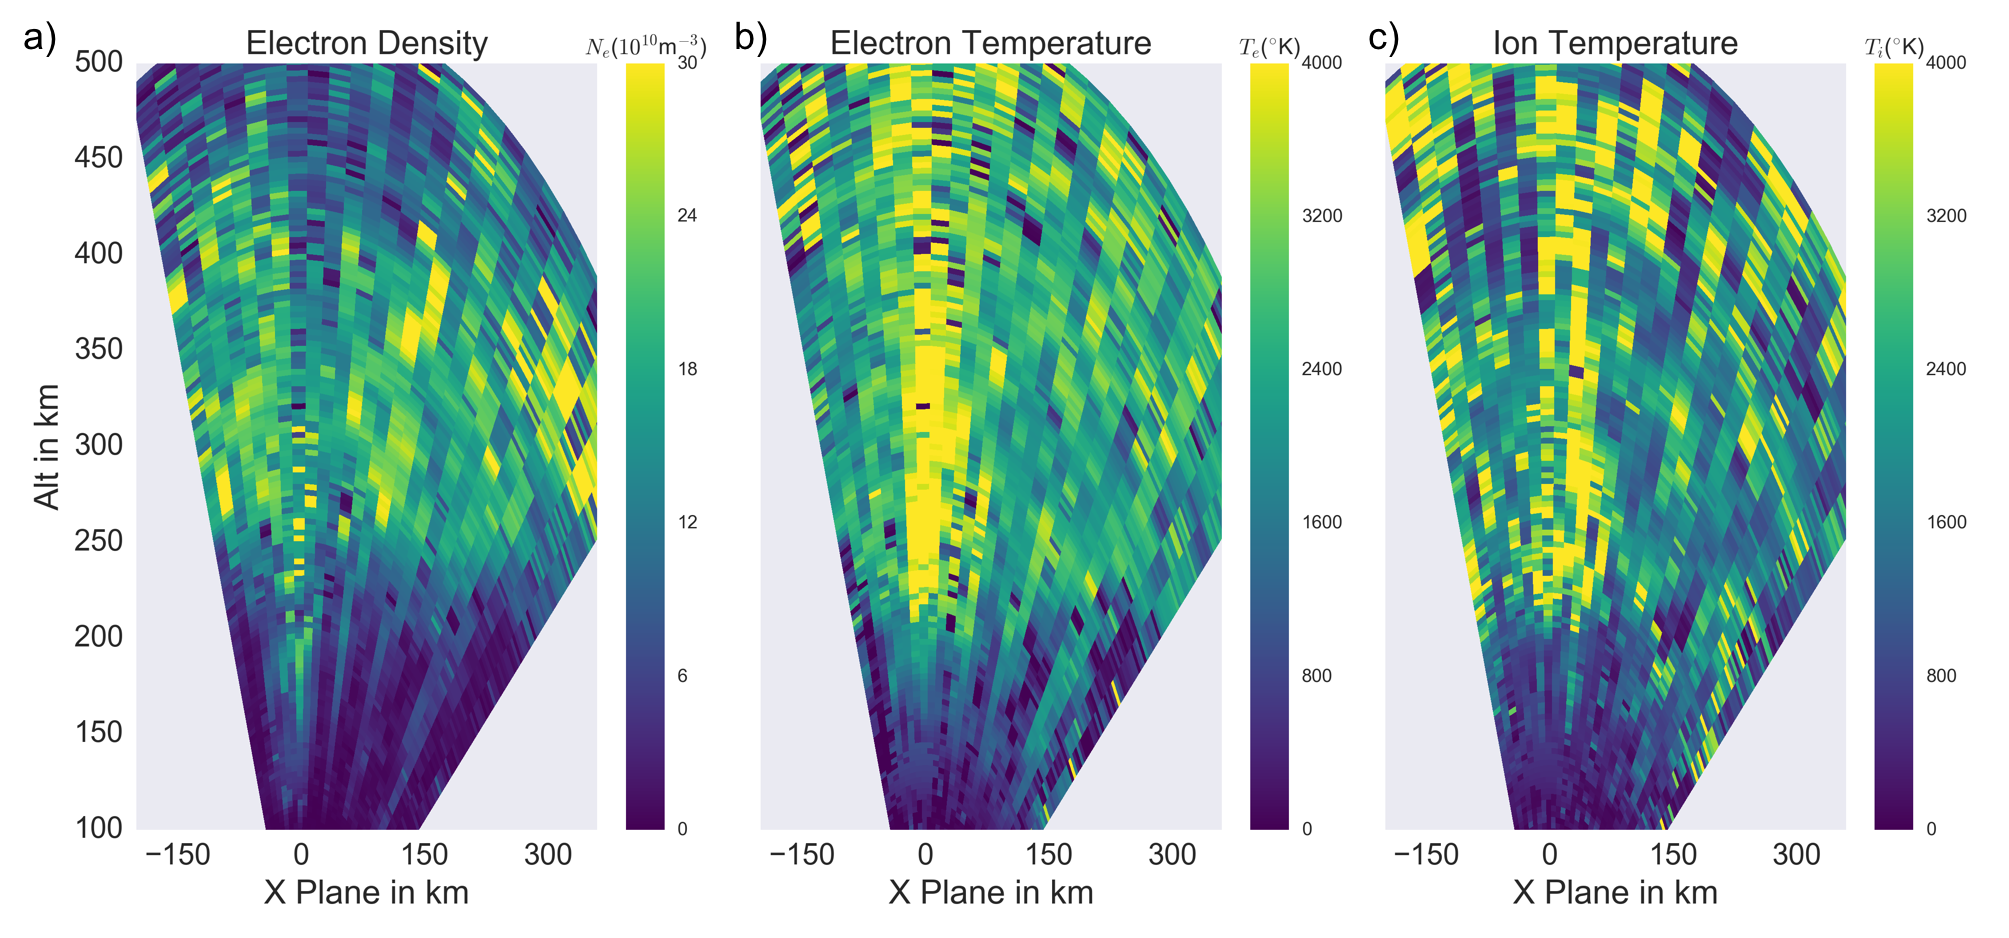
\includegraphics[width=6in]{0960_60_int}
\caption{Fitted Plasma Parameters at $t=960$ s with 60 second integration.}
%JOHN:  need to label these A,  B, C
\label{fig:fplparamst60}
\end{figure}

\begin{figure}[!t]
\centering
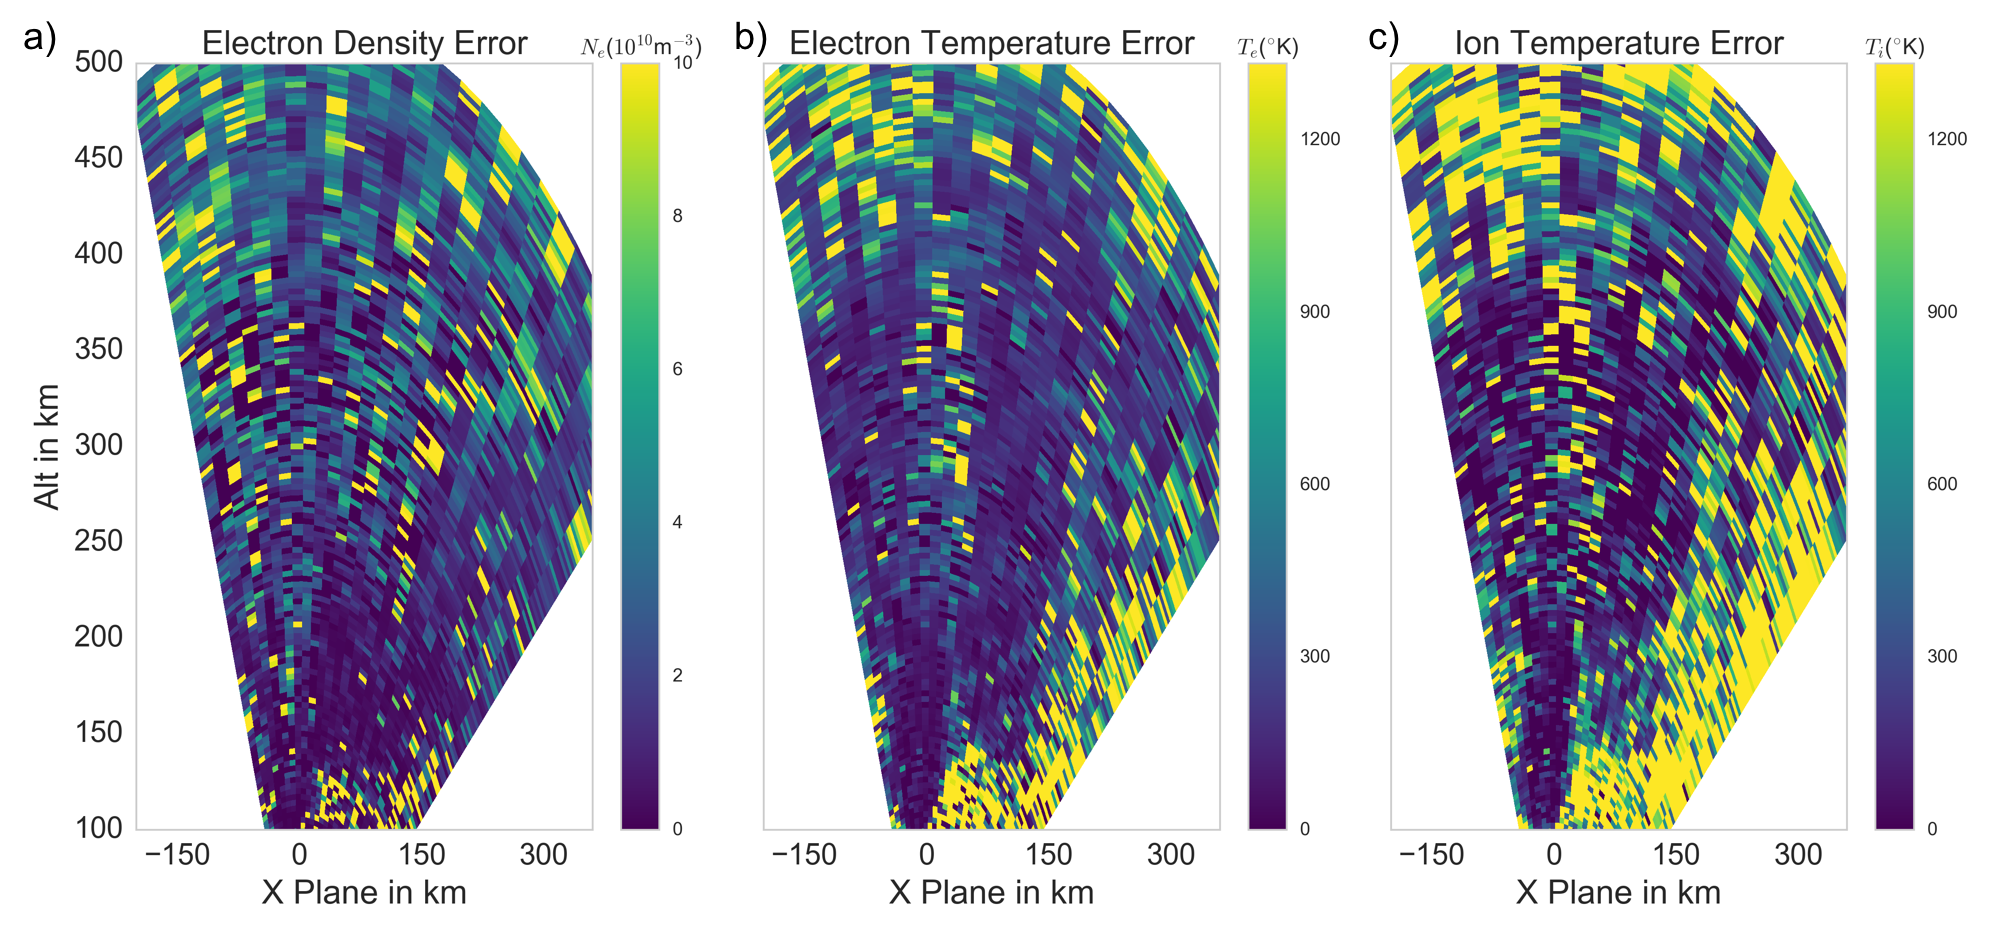
\includegraphics[width=6in]{0960_60_int_err}
\caption{Estimated errors from fitted Plasma Parameters at $t=960$ s with 60 second integration.}
\label{fig:fplparamst60err}
\end{figure}
%%%%%%%%%%%%%%%%%%%%%%%%%%%%%%%%%%%%%%%%%%%%%%%%%%%%%%%%%%%%%%%%%%%%%%%%%%%%%%%%%%%%%%%%%%
\section{Conclusion}
We have constructed a simulation of the full ISR measurement process, incorporating ESA radar capabilities and the full radar space-time ambiguity along with inherent ISR error sources, referred to as STISRS. Possible uses for STISRS in the research community have also been discussed and examples have been shown. These examples show how one can use the simulator to create large statistical data sets and also to more optimally design ionospheric radar experiments in the ISR space within the inherently large number of free parameters afforded by the radar control parameters. 

Development of the simulator will continue by adding new radar waveform modes, as currently only Barker code and uncoded single pulse modulations are available at this time. The simulator can also be used to create synthetic data for traditional single antenna based systems as well. Other possible expansions of the simulator include capability to calculate returns from each receiver element in a ESA based ISR system, such as the planned architecture of EISCAT-3D, and multi-static radar capabilities. These future additions will increase the simulator's value to designers who wish to more optimally exploit the capabilities of new systems. 

A more immediate application of this simulator can aid researchers in experiment planning. There are a number of phenomena that change on very small spatio-temporal scales, e.g. at high latitudes, and capturing observations of them would greatly benefit from optimization of the experiment set up. Researchers would be able iterate through different set ups for their experiments instead only being able to pick one just hope for the best. The ability of STISRS to directly create complex receiver voltage data provides a significant and novel capability, as some phenomena, such as those that have time scales on the order of an interpulse period, can only be observed at this data level. By releasing this simulation to the community, we hope that other researchers can find utility in it as they plan experiments or to understand observed radar data. 

%%%%%%%%%%%%%%%%%%%%%%%%%%%%%%%%%%%%%%%%%%%%%%%%%%%%%%%%%%%%%%%%%%%%%%%%%%%%%%%%%%%%%%%%%%
\begin{acknowledgments}
This work was supported by the National Science Foundation, through Aeronomy Program Grant AGS-1339500 to Boston University and Cooperative Agreement AGS-1242204 between the NSF and the Massachusetts Institute of Technology, and by the Air Force Office of Scientific Research under contract FA9550-12-1-018.   The authors are grateful to the International Space Science Institute (ISSI, Bern, Switzerland) for sponsoring a series of workshops from which the idea for this work emerged. Work at ERAU was supported by NSF grant AGS-1339537

Software used to create figures for this publications can be found at https://github.com/jswoboda/. Please contact the corresponding author, John Swoboda at swoboj@bu.edu, with any questions regarding the software along with any requests for the specific data used for the figures. \end{acknowledgments}


\bibliographystyle{BibTeX/agufull08}
\bibliography{BibTeX/litreview}
\end{article}

\end{document}

